\documentclass{article}

\usepackage{graphicx}
\usepackage{amssymb}
\usepackage{subcaption}
\usepackage{float}
\usepackage{gensymb}
\usepackage{amsmath}
\usepackage{array}
\usepackage{geometry}
 \geometry{
 a4paper,
 total={170mm,257mm},
 left=20mm,
 top=20mm,
 }
\usepackage{listings}

\title{IMAU-ICE / UFEMISM documentation}
\date{2022-03-16}
\author{C. J. Berends, J. A. Bernales}

\begin{document}
  \pagenumbering{gobble}
  \maketitle

  \begin{figure}[H]
    \centering
    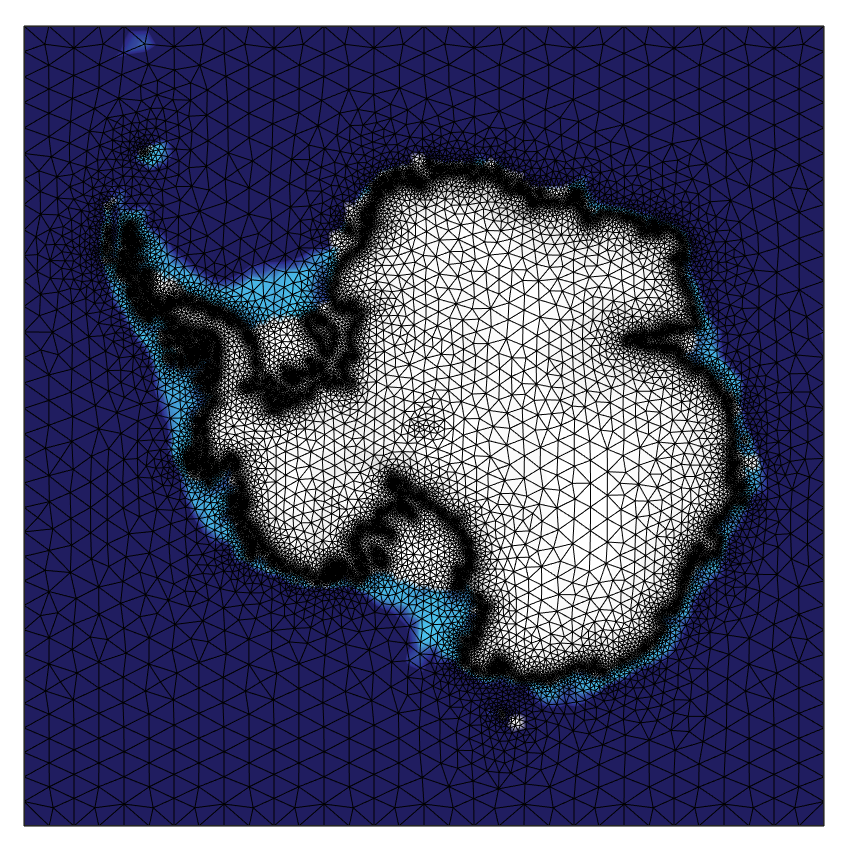
\includegraphics[width=0.8\linewidth]{Fig_UFEMISM.png}
  \end{figure}  

  \paragraph{Abstract}
  
IMAU-ICE and UFEMISM are the two ice-sheet models developed at the Institute for Marine and Atmospheric research Utrecht (IMAU). Both are so-called "shallow" models, solving a vertically-integrated approximation of the stress balance. The single difference between the two models is the grid; whereas IMAU-ICE uses a traditional square grid, UFEMISM uses a dynamic adaptive grid, with a high-resolution area near the grounding-line that adapts over time to the evolving ice-sheet geometry. While chiefly intended for palaeoglaciological applications, both models also provide support for future projections of ice-sheet retreat, as well as for schematic experiments of idealised-geometry ice sheets. This document aims to describe both models in their entirety, stating the underlying physical equations and deriving the discretised versions that are solved numerically, describing the code and data structure of the models, and providing instructions for both novice users and experienced developers.
  
\newpage
\tableofcontents

\newpage
\pagenumbering{arabic}
\part{Overview}

\section{Instructions for new users}

\textit{Basically just tell them to clone stuff from Github. Not that hard is it.}

\newpage
\section{Introduction}

\subsection{Background}

The Institute for Marine and Atmospheric research Utrecht (IMAU) has a long, rich history of ice-sheet modelling. In the early 2000's, GRICE (GReenland ICE-sheet model) was created: an SIA-only model   for studying the evolution of the Greenland ice sheet during glacial cycles. Several years later this model was adapted for the Antarctic ice sheet, including a module that solved the SSA for floating ice shelves, thus becoming ANICE (ANtarctic ICE-sheet model). Around 2010 this was extended into the coupled model ANICE-SELEN, which included four copies of ANICE to simulate the large continental Pleistocene ice-sheets (North America, Eurasia, Greenland, and Antarctica), as well as the sea-level equation solver SELEN. In early 2021 ANICE was replaced by its spiritual successor IMAU-ICE; still a square-grid hybrid SIA/SSA model, but thoroughly cleaned up and restructured, so as to enable a new generation of PhD's and postdocs to use and develop it without having to first know all the details and peculiarities of the work of their numerous predecessors.\\
\\
In the late 00's and early 10's, several studies were published that showed that the phenomenon of grounding-line migration was much more important for large-scale ice-sheet evolution then previously thought, particularly in Antarctica. They also showed that the increasingly common hybrid SIA/SSA ice models (like ANICE and IMAU-ICE) performed poorly at capturing this phenomenon, partly due to their often coarse resolution. The first few of these studies suggested that, in order to solve the problem, a resolution of 100 m or less was required. This is completely unachievable for palaeo-ice-sheet models; they must be able to simulate tens or sometimes hundreds of thousands of years, which is why researchers typically use resolutions of 10 - 40 km. However, several later studies developed clever ''heuristic'' solutions to this problem, which allowed them to use much coarser resolutions (ranging from 1 km to 20 km, depending on which study you believe) and still get good results. Aside from these numerical issues with resolution, it also became clear that small-scale topographical features like fjords and underwater hills could significantly affect large-scale ice-sheet dynamics, implying that even the ''heuristic'' models would still need a resolution of a few kilometres or less.\\
\\
However, while 20 km is still manageable, 10 km is already pushing the limits of what can reasonably be done with a square-grid model, and the even finer numbers required for resolving bed topography are simply not feasible for long palaeo-simulations. The obvious solution to this, in our view, was not to use a square grid. The studies that investigated the resolution problem already noted that in order to get good results, a high resolution was required only at the grounding line, not everywhere on the ice sheet. This intuitively makes sense; surface curvature (the leading term in the truncation error of any first-order discretisation scheme) is highest near the grounding line, as are the strain rates in the ice. Also, since grounded ice is thinnest and fastest there, this is where the topographical features of the underlying bedrock become most important. By creating a grid that has a high resolution only at the grounding line and nowhere else, you can ''skip'' a lot of non-essential calculations in the interior (determining velocities for essentially stagnant ice), freeing up computation time for the rest of the model. This line of reasoning led to the inception of UFEMISM: the first palaeo-ice-sheet model to use a dynamic adaptive grid.

\newpage
\subsection{Status quo}

\subsubsection{Features}

For each model component, different options are available, which can be selected through the config file. The different options are all explained in detail in the Physics part of the documentation.

\paragraph{Ice dynamics}
The stress balance can be solved using the SIA, the SSA, the hybrid SIA/SSA, or the DIVA. The thickness equation can be solved either explicitly or (semi-)implicitly. Time-stepping is by default done using a predictor/corrector scheme; for the hybrid SIA/SSA, an asynchronous scheme based on the CFL and advective stability criteria is also available. Proper grounding-line dynamics are achieved by using a sub-grid friction-scaling scheme; the grounding-line flux condition previously included in UFEMISM v1.0 is no longer available.

\paragraph{Sliding}
Currently the following sliding laws are available: Weertman, Coulomb, regularised Coulomb, Tsai2015, Schoof2005, and Zoet-Iverson. Bed roughness and basal hydrology are calculated using the bedrock elevation-dependent parameterisations by Martin et al. (2011).

\paragraph{Calving}
Currently, only a simple threshold-thickness calving law is included.

\paragraph{Thermodynamics}
A version of the heat equation is solved that includes vertical and horizontal advection, vertical (but not horizontal) diffusion, internal strain heating, basal frictional heating, and geothermal heat flux.

\paragraph{Climate}
The climate, described by monthly mean values of temperature and precipitation, is calculated from a combination of observational  data and GCM output using a matrix method, which accounts for changes in CO2, the ice-albedo feedback, and the elevation-temperature feedback. Optionally, a direct (transient) climate forcing can be prescribed.

\paragraph{Ocean}
3-D ocean temperature and salinity are calculated from a combination of observational data and GCM output using a matrix method. The data is extrapolated into the shelf cavity using the ISMIP6 protocol.

\paragraph{Surface mass balance}
The surface mass balance is calculated from the provided temperature and precipitation using the IMAU-ITM SMB model. This relatively simple insolation-temperature model constitutes a compromise between positive-degree-day (PDD) schemes and energy-balance models (EBM), and calculates the firn layer thickness and albedo, the rain/snow-fraction, and the different mass balance components. Optionally, a direct (transient) SMB forcing can be prescribed.

\paragraph{Basal mass balance}
The basal mass balance can be calculated using the three local parameterisations by Favier2019 (linear, quadratic, semi-quadratic), with the PICO model, with the Lazeroms 2019 plume model, or with PICOP (which combines these two). Near the grounding line, basal melt can be scaled using the NMP, FCMP, or PMP sub-grid schemes.

\paragraph{GIA}
GIA can be modelled using a simple ELRA model, or with the sea-level equation solver SELEN.

\paragraph{Isotopes}
The vertically-averaged englacial isotope content is calculated using a simple advection scheme.

\paragraph{Forcing}
The model can be forced using (ice-core) CO2 records, or with benthic oxygen isotope records using the inverse method.

\newpage
\subsubsection{Software}

\paragraph{Packages}
Both models require the following packages to compile and run: NetCDF, MPI, Lapack, and PETSc.

\paragraph{Data formats}
Both models write their output to NetCDF files. Spatial data fields are written to the \textsc{restart} and the \textsc{help\textunderscore fields} files. The \textsc{restart} file, as the name suggests, contains all the data fields required to initialise a new model run (ice thickness, englacial temperature, bed deformation, etc.). The \textsc{help\textunderscore fields} file can contain any number of configurable data fields; nearly a hundred different data fields can be selected (see the \textsc{write\textunderscore help\textunderscore field} subroutine in the \textsc{netcdf\textunderscore module} for the full list).\\
\\
For UFEMISM, both the \textsc{restart} and the \textsc{help\textunderscore fields} file come in a \textsc{mesh} and a \textsc{grid} variaty; the \textsc{mesh} variety provides data on the model mesh (which changes over time), whereas the \textsc{grid} variety is defined on a regular grid (resolution configurable) for quick and easy processing.

\subsubsection{Performance}

\textit{Just copy this from the old documentation until we get a chance to do some new performance tests.}

\paragraph{Speed}
\paragraph{Memory}

\newpage
\subsubsection{Development}

At the time of writing (March 2022), the following improvements are being developed.

\paragraph{Calving}
The threshold-thickness calving implementation is outdated. Jorge Bernales, Tijn Berends, and Lennert Stap are involved in CalvingMIP, wich aims to create a set of standardised experiments to verify and validate different calving laws. We expect that this will produce an improved calving implementation in IMAU-ICE and UFEMISM by late 2022 or possibly early 2023.

\paragraph{Isotopes}
The "ANICE legacy" advective transport scheme for calculating the englacial isotope content is outdated. We plan to replace this in UFEMISM with the Parcels package; this project is expected to start in late 2023.

\paragraph{Climate forcing}
A project is currently underway to improve the climate matrix method, so that it can be used with all the data from the PMIP3 and PMIP4 palaeoclimate projects. This is expected to yield results in late 2022.

\paragraph{Parallelisation}
A project is currently underway to extend the parallelisation of UFEMISM to a fully distributed architecture. Whereas the model is currently limited to using only a single node (typically up to 32 cores), when this project is finished this limitation will be removed, allowing the model to be run on any number of nodes. This will allow us to run full glacial cycles simulations with a grounding-line resolution as fine as 1 km. The is expected to be finished in late 2022.

\newpage
\section{Benchmark experiments}

A large number of benchmark experiments is included in the models. Config files to run all of these experiments, and scripts to process and analyse the data, and compare the results to analytical solutions or model ensembles, are contained in the Github repositories

\subsection{Halfar dome}

Halfar (1981) derived an analytical solution to the SIA for the case of a radially symmetrical, isothermal ice sheet lying on an undeformable flat bed. Typically, this experiment is run for 100,000 years, and the margin radius over time is compared to the analytical solution.

\begin{figure}[H]
  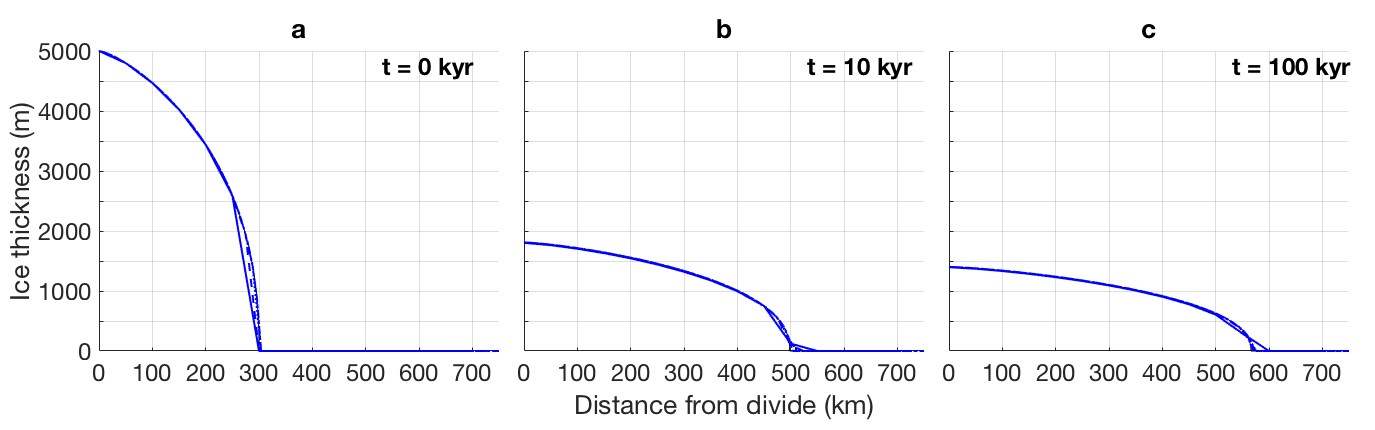
\includegraphics[width=0.95\linewidth]{Fig_benchmark_Halfar1.png}
  \caption{Cross-section of the ice sheet in the Halfar dome experiment at t = 0, t = 10,000 yr, and t = 100,000 yr, as simulated with IMAU-ICE.}
\end{figure}

\begin{figure}[H]
  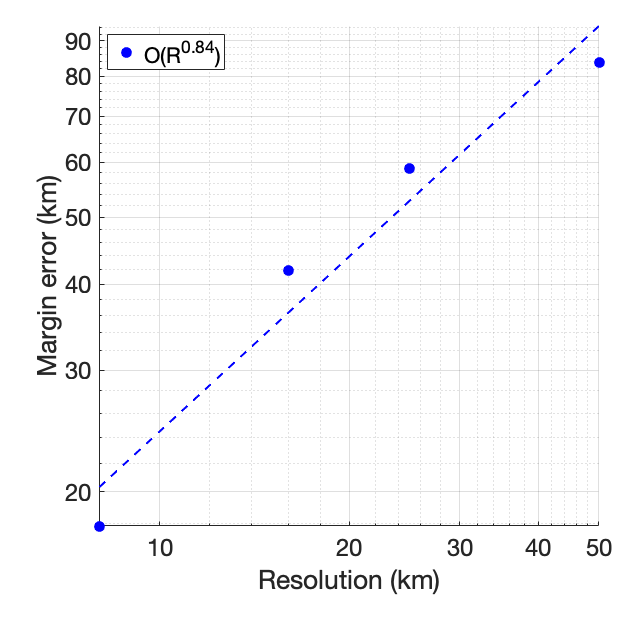
\includegraphics[width=0.4\linewidth]{Fig_benchmark_Halfar2.png}
  \caption{Error in simulated ice margin position at t = 100,000 yr in the Halfar dome experiment, as simulated with IMAU-ICE.}
\end{figure}

\subsection{Bueler dome}

Bueler et al. (2005) expanded the solution by Halfar (1981) to include a non-zero mass balance, leading to an ice-sheet that grows over time. Typically, this experiment is run from t = 2,000 to 12,000 years (at t = 0 the analytical solution for the mass balance approaches infinity, hence the starting time), and the margin radius over time is compared to the analytical solution.

\begin{figure}[H]
  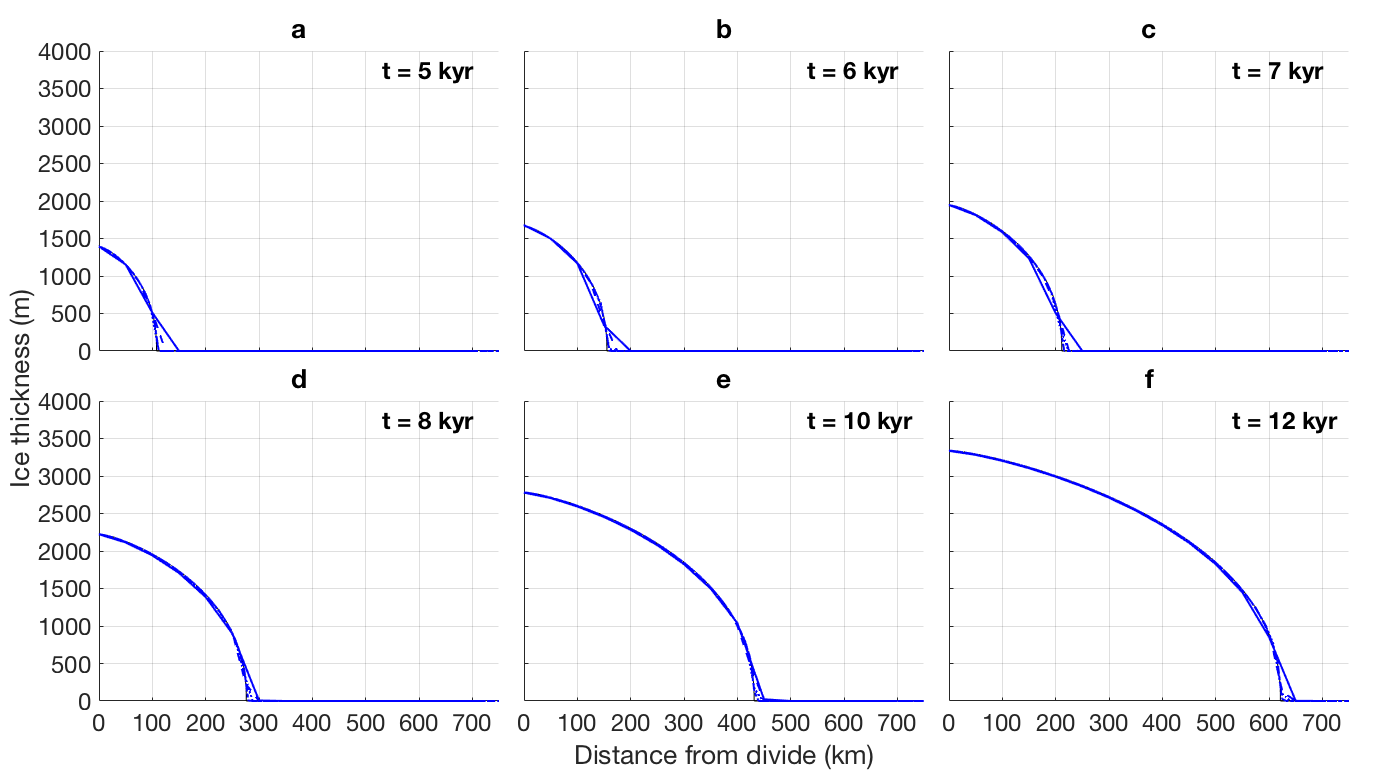
\includegraphics[width=0.95\linewidth]{Fig_benchmark_Bueler1.png}
  \caption{Cross-section of the ice sheet in the Bueler dome experiment at different times, as simulated with IMAU-ICE}
\end{figure}

\begin{figure}[H]
  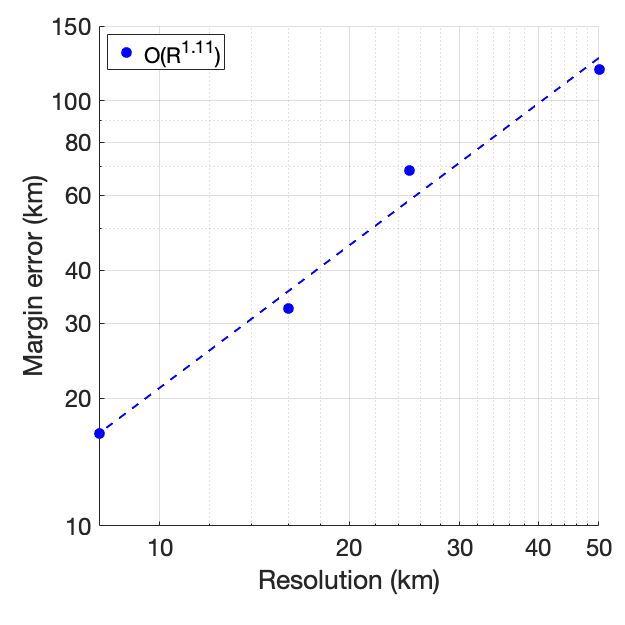
\includegraphics[width=0.4\linewidth]{Fig_benchmark_Bueler2.png}
  \caption{Error in simulated ice margin position at t = 12,000 yr in the Bueler dome experiment, as simulated with IMAU-ICE.}
\end{figure}

\subsection{SSA ice stream}

Schoof (2006) derived an analytical solution to the SSA for the case of an infinite, isothermal ice slab lying on an inclined plane with a single narrow strip of reduced basal slipperiness running in the downhill direction, leading to the formation of an ice stream. No along-flow variation exists; assuming the plane slopes down in the positive x-direction, the solution gives the x-component of the velocity $u$ as a function of $y$. The solution describes the velocity for a fixed geometry; no time evolution is included. The velocity solution can be directly compared to the analytical solution by Schoof.

\begin{figure}[H]
  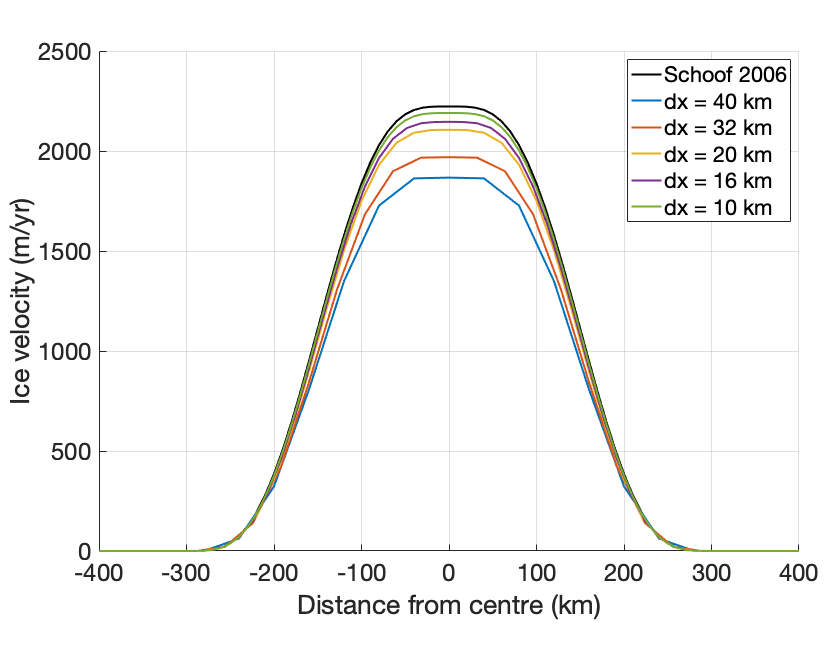
\includegraphics[width=0.5\linewidth]{Fig_benchmark_SSA_icestream.png}
  \caption{Downstream velocity $u$ as a function of the cross-stream coordinate $y$ in the SSA ice stream experiment, compared to the analytical solution by Schoof (2006), as simulated with IMAU-ICE.}
\end{figure}

\subsection{EISMINT-1}

The first set of experiments from the European Ice-Sheet Modelling INiTiative (EISMINT; Huybrechts et al., 1996) concern a radially symmetric ice-sheet lying on a flat, undeformable bed. The surface mass balance is described using a simple, spatially and temporally variable parameterisation, which leads to the ice sheet growing and shrinking over either 20-kyr or 40-kyr glacial cycles. The englacial temperature is calculated, but does not affect the ice rheology; the flow factor is kept constant and uniform. The calculated ice thickness and basal temperature at the ice divide can be compared to the model ensemble from Huybrechts et al. (1996).

\begin{figure}[H]
  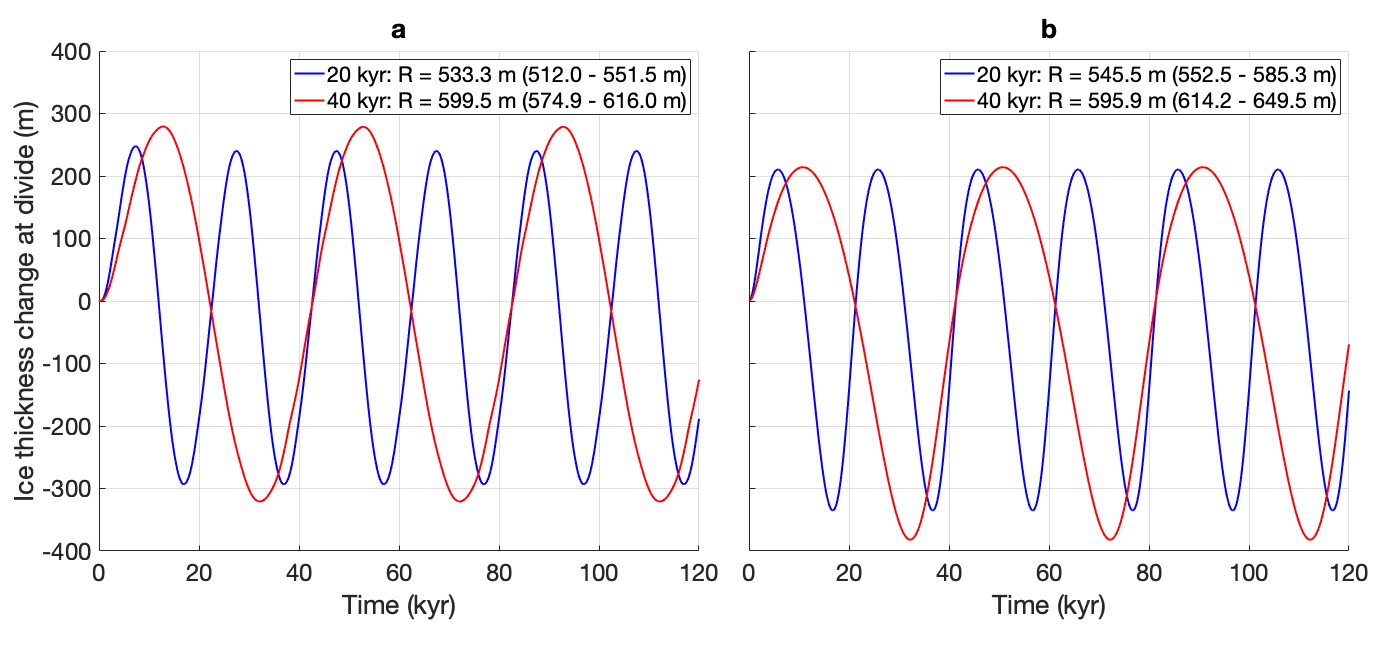
\includegraphics[width=0.95\linewidth]{Fig_benchmark_EISMINT1.png}
  \caption{Ice thickness at the divide over time for the “glacial cycle” experiments from the first EISMINT intercomparison exercise, with a moving margin (panel a) and a fixed margin (panel b). The legends list the simulated glacial-interglacial difference R for the 15 last cycle, with the range of numbers reported by Huybrechts et al. (1996) listed between brackets for comparison. Results produced with IMAU-ICE.}
\end{figure}

\begin{figure}[H]
  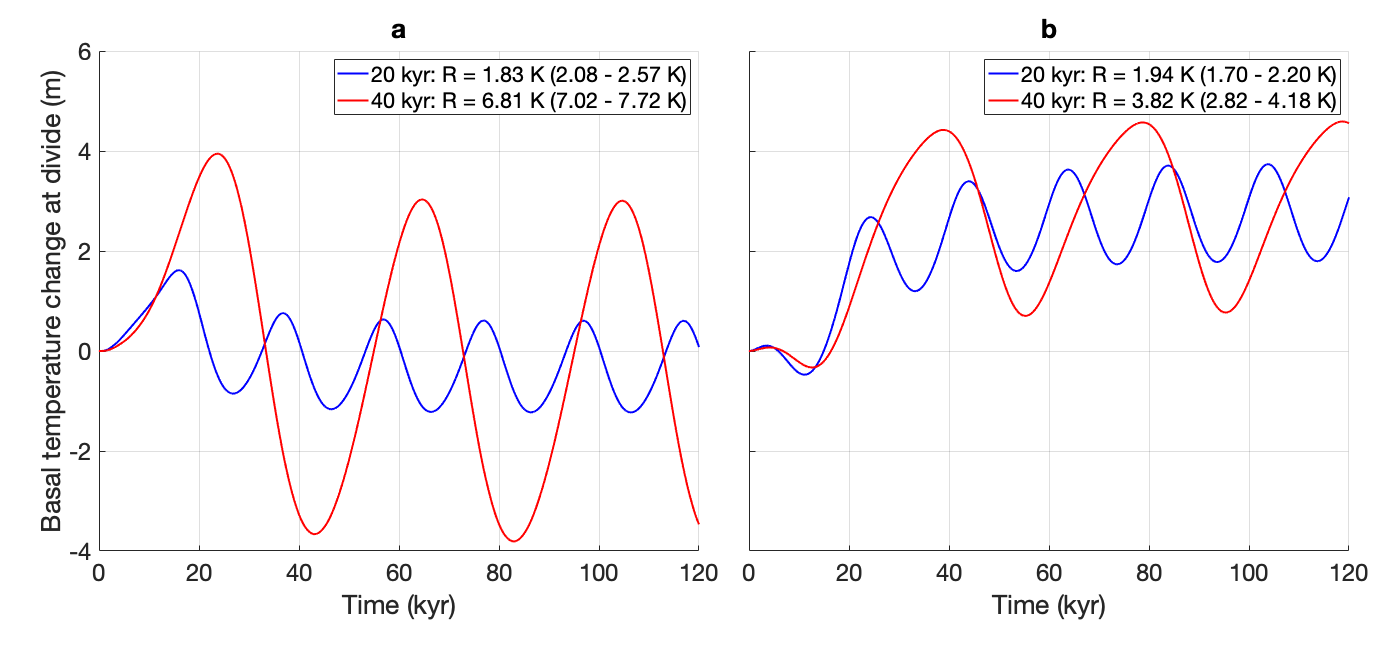
\includegraphics[width=0.95\linewidth]{Fig_benchmark_EISMINT2.png}
  \caption{Ice temperature at the base of the ice divide, relative to the pressure melting point, over time for the “glacial cycle” experiments from the first EISMINT intercomparison exercise, with a moving margin (panel a) and a fixed margin (panel b). The legends list the simulated glacial-interglacial difference R for the last cycle, with the range of numbers reported by Huybrechts et al. (1996) listed between brackets for comparison. Results produced with IMAU-ICE.}
\end{figure}

\subsection{ISMIP-HOM}

The Ice-Sheet Model Intercomparison Project for Higher-Order Models (ISMIP-HOM; Pattyn et al., 2008) describes a set of idealised ice-sheet geometries with increasingly high aspect ratios, so that the solutions from lower-order (e.g. vertically averaged) approximations to the stress balance become increasingly inaccurate. The calculated 3-D velocity profile can be compared to the model ensemble, showing that the hybrid SIA/SSA solution rapidly diverges from the full-Stokes solution, whereas the DIVA remains close to it at much higher aspect ratios.

\begin{figure}[H]
  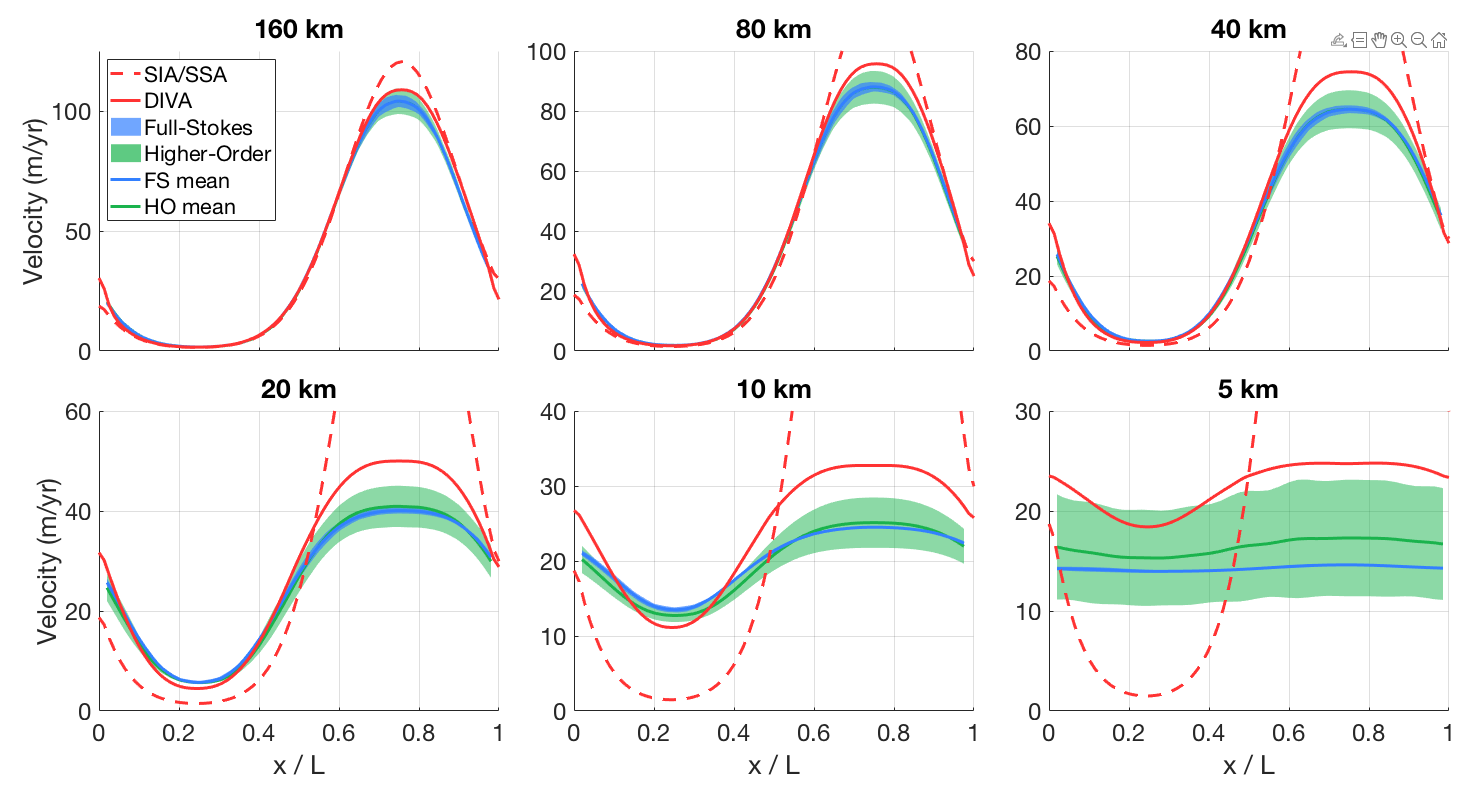
\includegraphics[width=0.95\linewidth]{Fig_benchmark_ISMIP_HOM_A.png}
  \caption{Modelled surface velocity transects for all versions of ISMIP-HOM experiment A (infinite ice slab on a sloping bed with sinusoid bumps in both directions), calculated with both the hybrid SIA/SSA (red dashed line) and the DIVA (red solid line). The results of the higher-order models (green) and the full-Stokes models (blue) that participated in ISMIP-HOM are shown for comparison. Results produced with IMAU-ICE.}
\end{figure}

\begin{figure}[H]
  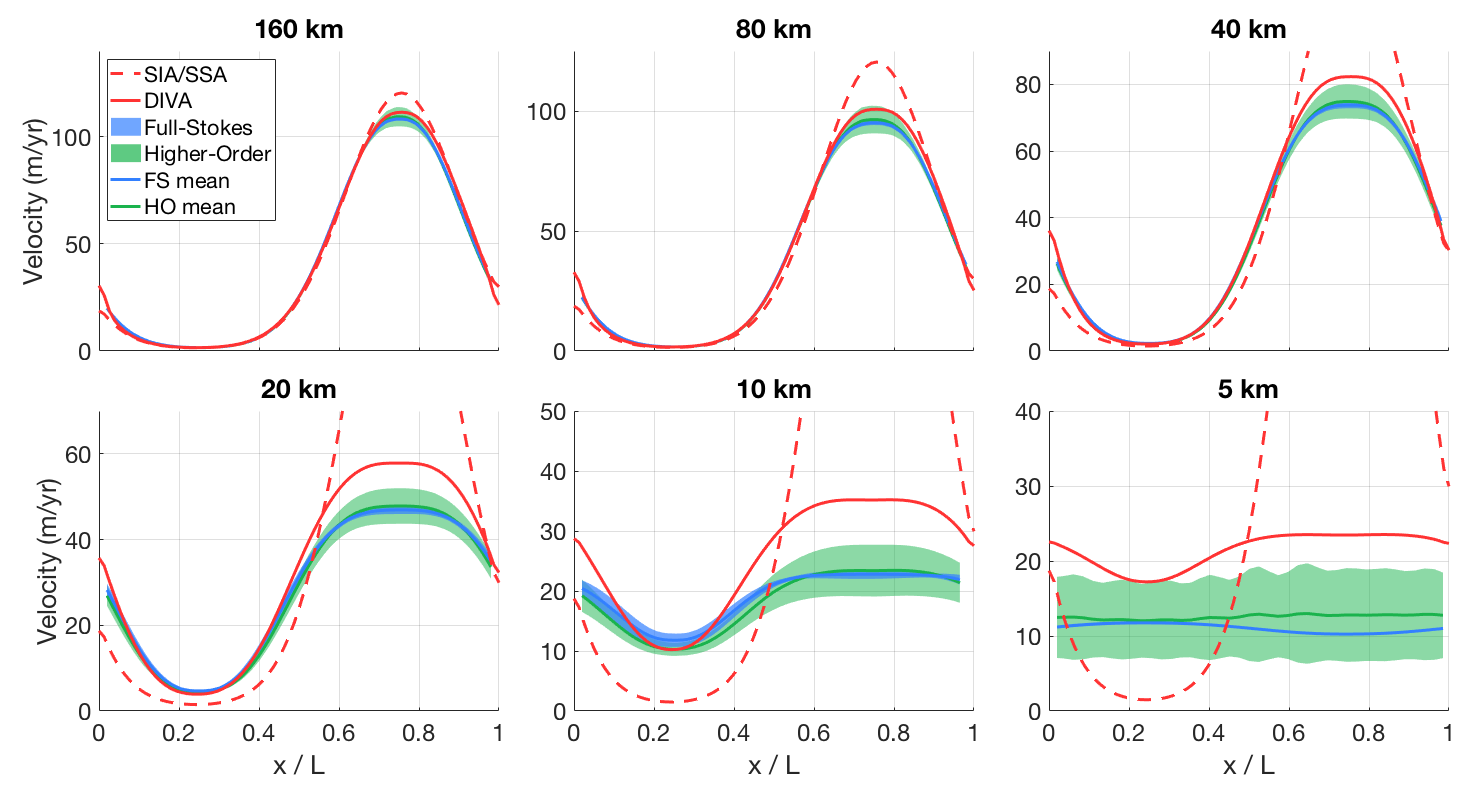
\includegraphics[width=0.95\linewidth]{Fig_benchmark_ISMIP_HOM_B.png}
  \caption{Modelled surface velocity transects for all versions of ISMIP-HOM experiment B (infinite ice slab on a sloping bed with sinusoid bumps in one direction), calculated with both the hybrid SIA/SSA (red dashed line) and the DIVA (red solid line). The results of the higher-order models (green) and the full-Stokes models (blue) that participated in ISMIP-HOM are shown for comparison. Results produced with IMAU-ICE.}
\end{figure}

\begin{figure}[H]
  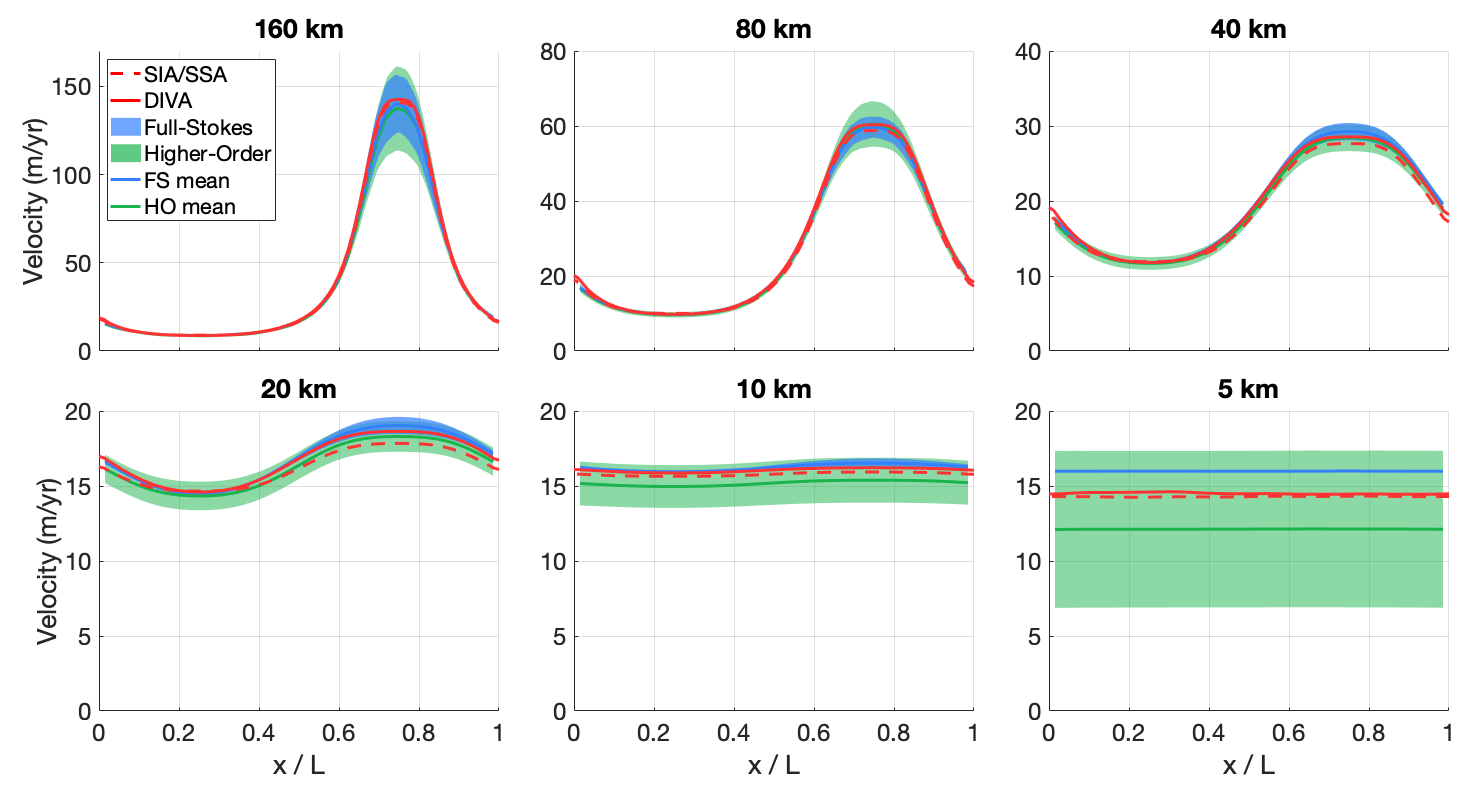
\includegraphics[width=0.95\linewidth]{Fig_benchmark_ISMIP_HOM_C.png}
  \caption{Modelled surface velocity transects for all versions of ISMIP-HOM experiment C (infinite ice slab on a sloping bed with oscillating friction in both directions), calculated with both the hybrid SIA/SSA (red dashed line) and the DIVA (red solid line). The results of the higher-order models (green) and the full-Stokes models (blue) that participated in ISMIP-HOM are shown for comparison. Results produced with IMAU-ICE.}
\end{figure}

\begin{figure}[H]
  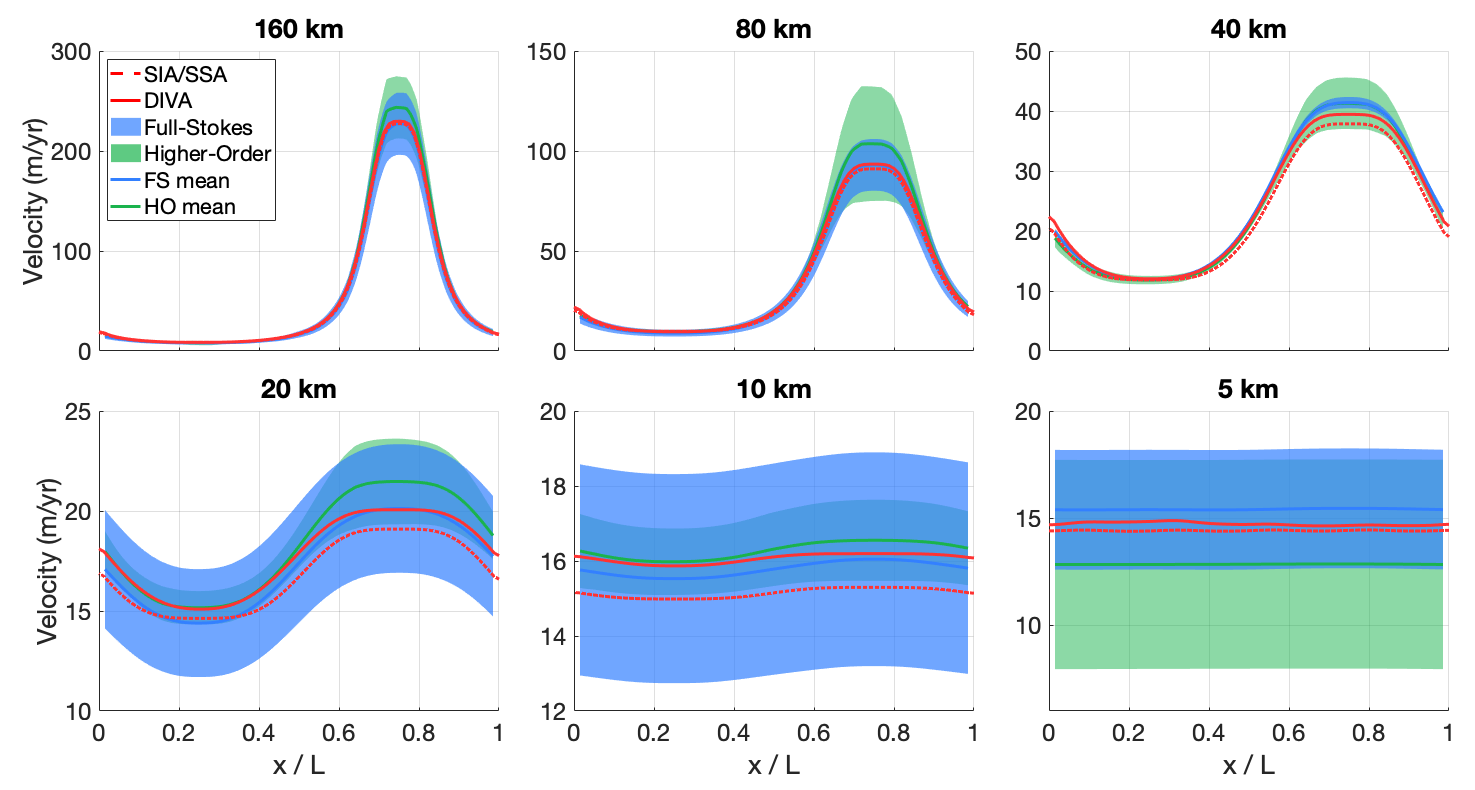
\includegraphics[width=0.95\linewidth]{Fig_benchmark_ISMIP_HOM_D.png}
  \caption{Modelled surface velocity transects for all versions of ISMIP-HOM experiment D (infinite ice slab on a sloping bed with oscillating friction in one direction), calculated with both the hybrid SIA/SSA (red dashed line) and the DIVA (red solid line). The results of the higher-order models (green) and the full-Stokes models (blue) that participated in ISMIP-HOM are shown for comparison. Results produced with IMAU-ICE.}
\end{figure}

\begin{figure}[H]
  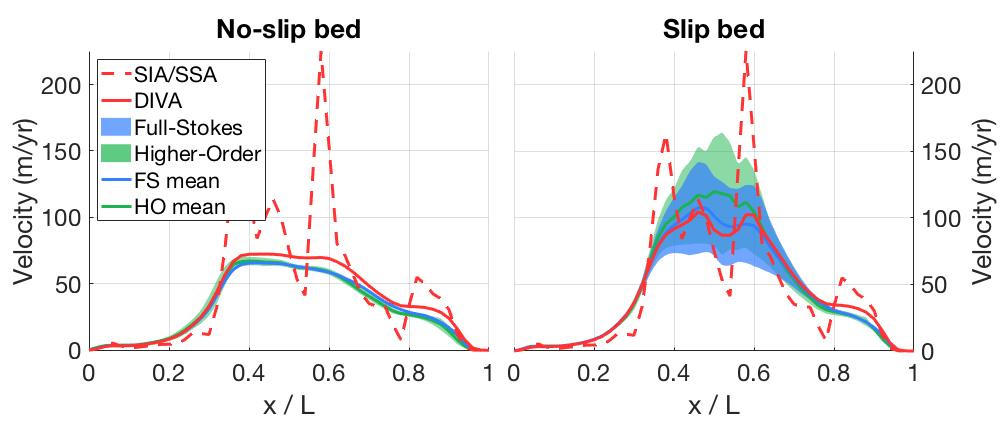
\includegraphics[width=0.7\linewidth]{Fig_benchmark_ISMIP_HOM_E.png}
  \caption{Modelled surface velocity transects for both versions of ISMIP-HOM experiment E (Haut Glacier d’Arolla, with and without a slippery bed region), calculated with both the hybrid SIA/SSA (red dashed line) and the DIVA (red solid line). The results of the higher-order models (green) and the full-Stokes models (blue) that participated in ISMIP-HOM are shown for comparison. Results produced with IMAU-ICE.}
\end{figure}

\begin{figure}[H]
  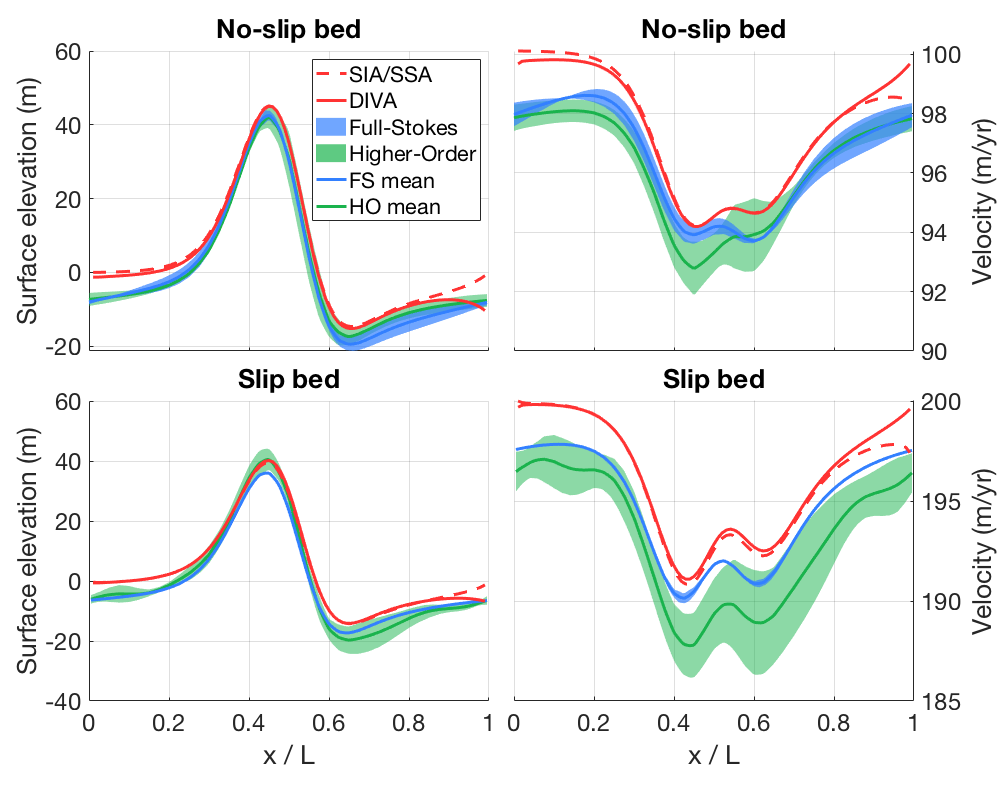
\includegraphics[width=0.7\linewidth]{Fig_benchmark_ISMIP_HOM_F.png}
  \caption{Modelled surface elevation and velocity transects for both versions of ISMIP-HOM experiment F (infinite ice slab on a sloping bed with a single Gaussian bump, with and without a slippery bed), calculated with both the hybrid SIA/SSA (red dashed line) and the DIVA (red solid line). The results of the higher-order models (green) and the full-Stokes models (blue) that participated in ISMIP-HOM are shown for comparison. Results produced with IMAU-ICE.}
\end{figure}

\subsection{MISMIP}

The first Marine Ice-Sheet Model Intercomparison Project (MISMIP; Pattyn et al., 2012) describes a flowline of an ice-sheet lying on an inclined plane, with part of the domain being subaerial and part being submerged, leading to the formation of a marine ice sheet feeding into an infinite ice shelf. This experiment is (in)famous for showing that, although in this unbuttressed setting the SSA has a unique solution for any uniform flow factor, many models displayed significant hysteresis in the calculated grounding-line position. The original experiment described a flowline; to make this feasible for IMAU-ICE and UFEMISM, we followed Pattyn (2017) by adapting it to plan-view, by extruding the flowline radially. The experiment now describes a cone-shaped island, covered by a radially symmetric ice sheet and shelf.

\subsection{MISMIP+}

This schematic experiment, proposed by Asay-Davis et al. (2016) aims to study grounding-line retreat caused by increased melting or calving in a strongly buttressed geometry. The steady state describes an 80-km wide ice stream flowing into an embayed shelf, with the grounding line resting on a retrograde slope. Once the modelled ice sheet has equilibrated, sub-shelf melt is increased, causing the grounding-line to retreat, over a period of 100 years. After that, the experiment splits up, with one branch maintaining the melt for another 100 years, continuing the retreat, while the other stops the melt and produces a re-advance. The modelled grounding-line position over time can be compared to the model ensemble by Cornford et al. (2020).

\subsection{MISOMIP1}

This experiment concerns the same geometry as MISMIP+. Proposed by Asay-Davis et al. (2016), MISOMIP1 aims to intercompare coupled ice-sheet - ocean models. The experimental protocol prescribes a vertical ocean temperature and salinity profile at the domain boundary. This means that ice-sheet models with basal melt parameterisations that use these quantities (which is the case in IMAU-ICE and UFEMISM) can in principle perform the experiment as well. As in MISMIP+, the grounding-line position over time can be compared between models; however, the intercomparison has not yet been published.

\newpage
\section{Model structure}

\subsection{General}

\textit{Describe the coupling program, the four model regions, and the asynchronous coupling between the model components.}

\subsection{Data structure}

\textit{Explain about Fortran types.}

\subsection{Code structure}

\textit{Initialise, run, remap, with different versions for different options of model components.}

\newpage
\part{Physics}

\section{Ice dynamics}

IMAU-ICE and UFEMISM by default solve the Depth-Integrated Viscosity Approximation (DIVA) to calculate the ice velocities. The hybrid SIA/SSA, as well as only the SIA or SSA, is included as an alternative. The DIVA has been shown to be significantly more physically accurate than the hybrid SIA/SSA, at almost no additional computational expense.

\subsection{SIA}

The Shallow Ice Approximation (SIA) is arrived at by neglecting all stresses in the Stokes equations except those arising due to vertical shearing (i.e. $\frac{\partial u}{\partial z}$, $\frac{\partial v}{\partial z}$). This reduces the equations to the point where they can be solved analytically, which results in the following expression:

\begin{align} \label{eq:SIA_01}
D(z) &= 2 {\left( \rho g H \right)}^n {\left| \nabla H \right|}^{n-1} \int_0^z A \left( T^{\ast} \left( \zeta \right) \right) \zeta^n d\zeta, \\
u(z) &= D(z) \frac{\partial h}{\partial x}, \\
v(z) &= D(z) \frac{\partial h}{\partial y}.
\end{align}

Here, the vertical velocity profiles can be calculated using only local quantities (ice thickness, surface slope, viscosity profile), so that no differential needs to be solved. This makes the SIA a very computationally efficient approach. The general consensus is that the SIA is accurate for the interior of an ice sheet, but cannot accurately describe ice flow near the ice margin, near the grounding line, or in other areas where the local ice thickness is no longer negligibly small compared to the horizontal length scale of the local topography.\\
\\
As is the case in most ice-sheet models, both UFEMISM and IMAU-ICE solve the SIA on a staggered grid. This greatly improves numerical stability, and allows the use of much larger time steps (limited only by the CFL-criterion for diffusion equations) than would otherwise be the case. In IMAU-ICE, the Arakawa-C grid is used; in UFEMISM, velocities are calculated on the centres of the mesh triangles, equivalent to the Arakawa-B grid.\\
\\
The solution to the SIA can be verified by comparing to the analytical solution in the Halfar and Bueler dome experiments, or to the model ensemble in the EISMINT-1 intercomparison. When used as part of the hybrid SIA/SSA approach, it can also be verified in the ISMIP-HOM ensemble (though only in the large-scale cases).

\subsection{SSA}

The Shallow Shelf Approximation (SSA) follows from the Stokes equations when all stresses are neglected except for those arising from horizontal stretching and shearing (i.e. $\frac{\partial u}{\partial x}$, $\frac{\partial u}{\partial y}$, $\frac{\partial v}{\partial x}$, $\frac{\partial v}{\partial y}$), assuming that no vertical variations in velocity exist (i.e. $\frac{\partial u}{\partial z} = \frac{\partial v}{\partial z} = 0$). This approximation is generally agreed to be valid in fast-flowing ice streams and shelves. Writing the resulting stress balance in terms of velocity yields the following expression:

\begin{align} \label{eq:SSA_01}
\frac{\partial}{\partial x} \left[ 2 \overline{\eta} H \left( 2 \frac{\partial u}{\partial x} + 
\frac{\partial v}{\partial y} \right) \right] + 
\frac{\partial}{\partial y} \left[ \overline{\eta} H \left( \frac{\partial u}{\partial y} + 
\frac{\partial v}{\partial x} \right) \right] - \beta_b u &= -\tau_{d,x}, \\
\frac{\partial}{\partial y} \left[ 2 \overline{\eta} H \left( 2 \frac{\partial v}{\partial y} + 
\frac{\partial u}{\partial x} \right) \right] + 
\frac{\partial}{\partial x} \left[ \overline{\eta} H \left( \frac{\partial v}{\partial x} + 
\frac{\partial u}{\partial y} \right) \right] - \beta_b v &= -\tau_{d,y}.
\end{align}

The vertically averaged effective viscosity $\overline{\eta}$ is expressed in terms of the horizontal strain rates:

\begin{align} \label{eq:SSA_02}
\overline{\eta} &= \frac{1}{H} \int_b^s \eta(z) dz 
= \frac{1}{H} \int_b^s \frac12 A^{\frac{-1}{n}} \dot{\epsilon}_e^{\frac{1-n}{n}} dz, \\
{\dot{\epsilon}}_e &= {\left[ {\left( \frac{\partial u}{\partial x} \right) }^2 + {\left( \frac{\partial v}{\partial y} \right) }^2 + \frac{\partial u}{\partial x} \frac{\partial v}{\partial y} + \frac14 {\left( {\left( \frac{\partial u}{\partial y} \right) } + {\left( \frac{\partial v}{\partial x} \right) } \right)}^2 \right] }^{\frac12}.
\end{align}

Both the basal friction coefficient $\beta_b$ and the effective viscosity $\eta$ depend strongly non-linearly on the velocity $u$, making the SSA a non-linear PDE. Both IMAU-ICE and UFEMISM solve this problem iteratively; first, $\beta_b$ and $\eta$ are calculated for a certain initial guess of $u,v$ (usually simply zero). Then, \eqref{eq:SSA_01} is solved while keeping $\beta_b$ and $\eta$ constant (the so-called "linearised" problem). Then, $\beta_b$ and $\eta$ are calculated using the new solution for $u,v$, and \eqref{eq:SSA_01} is solved again, and so on and so forth, until a stable solution is reached.\\
\\
In earlier versions of the models (up to IMAU-ICE v1.1, and UFEMISM v1.1), the SSA was simplified using the so-called "sans approximation", introduced by Determann (1991) and popularised by Huybrechts (1992). In this approximation, horizontal gradients in the product term $N = \overline{\eta} H$ are neglected, simplifying \eqref{eq:SSA_01} to:

\begin{align} \label{eq:SSA_03}
4 \frac{\partial^2 u}{\partial x^2} + \frac{\partial^2 u}{\partial y^2} + 3 \frac{\partial^2 v}{\partial x \partial y}
- \frac{\beta_b u}{N} = \frac{-\tau_{d,x}}{N}, \\
4 \frac{\partial^2 v}{\partial y^2} + \frac{\partial^2 v}{\partial x^2} + 3 \frac{\partial^2 u}{\partial x \partial y}
- \frac{\beta_b v}{N} = \frac{-\tau_{d,y}}{N}.
\end{align}

However, subsequent work has shown that this approximation, which was made by Determann for a shelf-only model, is inaccurate for grounded ice. It has therefore been removed from IMAU-ICE v2.0 and onwards, and UFEMISM v2.0 and onwards, although it is still available as an option.\\
\\
The solution to the SSA can be verified by comparing to the analytical solution in the Schoof (2006) ice-stream experiment. When used as part of the hybrid SIA/SSA approach, it can also be verified in the ISMIP-HOM ensemble (though only in the large-scale cases).

\subsection{Hybrid SIA/SSA}

In the hybrid SIA/SSA approach, developed by Bueler and Brown (2009) for PISM, the SIA and SSA are solved separately, and the resulting velocity fields are simply added together. This approach is still used in many ice-sheet models (e.g. SICOPOLIS; Greve et al., 2011; f.ETISh; Pattyn, 2017; GRISLI; Quiquet et al., 2018), as it is relatively simple to implement, and very computationally efficient.\\
\\
The solution to the hybrid SIA/SSA can be verified by comparing to the model ensemble in the large-scale experiments of ISMIP-HOM.

\subsection{DIVA}

The Depth-Integrated Viscosity Approximation (DIVA) can be derived by vertically integrated the Blatter-Pattyn approximation, which in turn follow from the Stokes equations by neglecting all stresses except those arising from horizontal stretching and shearing, and vertical shearing (i.e. $\frac{\partial u}{\partial x}$, $\frac{\partial u}{\partial y}$, $\frac{\partial v}{\partial x}$, $\frac{\partial v}{\partial y}$, $\frac{\partial u}{\partial z}$, $\frac{\partial v}{\partial z}$). This results in the following expression:

\begin{align} \label{eq:DIVA_01}
\frac{\partial}{\partial x} \left[ 2 \overline{\eta} H \left( 2 \frac{\partial \overline{u}}{\partial x} + 
\frac{\partial \overline{v}}{\partial y} \right) \right] + 
\frac{\partial}{\partial y} \left[ \overline{\eta} H \left( \frac{\partial \overline{u}}{\partial y} + 
\frac{\partial \overline{v}}{\partial x} \right) \right] - \beta_{\textrm{eff}} \overline{u} &= -\tau_{d,x}, \\
\frac{\partial}{\partial y} \left[ 2 \overline{\eta} H \left( 2 \frac{\partial \overline{v}}{\partial y} + 
\frac{\partial \overline{u}}{\partial x} \right) \right] + 
\frac{\partial}{\partial x} \left[ \overline{\eta} H \left( \frac{\partial \overline{v}}{\partial x} + 
\frac{\partial \overline{u}}{\partial y} \right) \right] - \beta_{\textrm{eff}} \overline{v} &= -\tau_{d,y}.
\end{align}

These equations are very similar to those of the SSA, with two differences. Firstly, they now concern the vertically \emph{ averaged} velocities $\overline{u}$, $\overline{v}$ instead of the vertically \emph{uniform} velocities $u$, $v$. Secondly, the basal friction coefficient $\beta_b$ has been replaced with the term $\beta_{\textrm{eff}}$, which contains terms describing both basal friction, and vertical shearing.\\
\\
The expression for the effective strain rate is slightly different as well, now also includes terms for vertical shearing, thus introducing a vertical variation:

\begin{equation} \label{eq:DIVA_02}
{\dot{\epsilon}}_e \left( z \right) = { \left[ {\left( \frac{\partial \overline{u}}{\partial x} \right) }^2 + {\left( \frac{\partial \overline{v}}{\partial y} \right) }^2 + \frac{\partial \overline{u}}{\partial x} \frac{\partial \overline{v}}{\partial y} + \frac14 {\left( {\left( \frac{\partial \overline{u}}{\partial y} \right) } + {\left( \frac{\partial \overline{v}}{\partial x} \right) } \right)}^2 + \frac14 \frac{\partial u \left( z \right)}{\partial z} + \frac14 \frac{\partial v \left( z \right)}{\partial z} \right] }^{\frac12}.
\end{equation}

The term $\beta_{\textrm{eff}}$ is defined as:

\begin{align} \label{DIVA_03}
\beta_{\textrm{eff}} &= \frac{\beta_b}{1 + \beta_b F_2}, \\
F_n &= \int_b^s \frac{1}{\eta \left( z \right)} {\left( \frac{s - z}{H} \right)}^n dz.
\end{align}

A comprehensive derivation of these equations is provided by Lipscomb et al. (2019).\\
\\
Due to their strong similarity, the same numerical solver can be used to solve both the linearised SSA and the linearised DIVA. The non-linear iteration solving $\beta_b$/$\beta_{\textrm{eff}}$ and $\eta$ is, of course, different.\\
\\
The solution to the DIVA can be verified in the ISMIP-HOM experiments, where it remains closer to the full-Stokes solution at significantly smaller scales than does the hybrid SIA/SSA.

\newpage
\subsection{Thickness equation}

In shallow ice models, ice thickness is integrated through time by solving a two-dimensional advection equation describing conservation of mass:

\begin{equation} \label{eq:thickness_01}
\frac{\partial H}{\partial t} = -\nabla \cdot \left( \textbf{u} H \right) + M.
\end{equation}

Here, the rate of change $\frac{\partial H}{\partial t}$ of the ice thickness $H$ is related to the divergence of the ice flux $\textbf{u} H$, and the net mass balance $M$.

\subsubsection{IMAU-ICE - explicit method}

By default, IMAU-ICE solves \eqref{eq:thickness_01} using an explicit scheme in time, and an upwind scheme for the ice flux divergence. Expanding the gradient operator in \eqref{eq:thickness_01} yields:

\begin{equation} \label{eq:thickness_02}
\frac{\partial H}{\partial t} = -\left( \frac{\partial \left( u H\right) }{\partial x} + \frac{\partial \left( v H\right) }{\partial y} \right) + M.
\end{equation}

Since the velocities $u,v$ are defined on the staggered Arakawa-C grid, using an upwind scheme yields the following discretised expression:

\begin{equation} \label{eq:thickness_03}
\begin{split}
\frac{\partial H^{i,j}}{\partial t} = \frac{-1}{\Delta} & \left[ 
\max \left( u^{i,j},0 \right) H^{i,j} + \min \left( u^{i,j},0 \right) H^{i+1,j} \right. - \\
& \left. \max \left( u^{i-1,j},0 \right) H^{i-1,j} - \min \left( u^{i-1,j},0 \right) H^{i,j} \right. + \\
& \left. \max \left( v^{i,j},0 \right) H^{i,j} + \min \left( v^{i,j},0 \right) H^{i,j+1} \right. - \\
& \left. \max \left( v^{i,j-1},0 \right) H^{i,j-1} - \min \left( v^{i,j-1},0 \right) H^{i,j} \right]
+ M^{i,j}.
\end{split}
\end{equation}

Discretising this expression explicitly in time then yields:

\begin{equation} \label{eq:thickness_04}
\begin{split}
\frac{H^{i,j,t+\Delta t} - H^{i,j,t}}{\Delta t} = \frac{-1}{\Delta} & \left[ 
\max \left( u^{i,j,t},0 \right) H^{i,j,t} + \min \left( u^{i,j,t},0 \right) H^{i+1,j,t} \right. - \\
& \left. \max \left( u^{i-1,j,t},0 \right) H^{i-1,j,t} - \min \left( u^{i-1,j,t},0 \right) H^{i,j,t} \right. + \\
& \left. \max \left( v^{i,j,t},0 \right) H^{i,j,t} + \min \left( v^{i,j,t},0 \right) H^{i,j+1,t} \right. - \\
& \left. \max \left( v^{i,j-1,t},0 \right) H^{i,j-1,t} - \min \left( v^{i,j-1,t},0 \right) H^{i,j,t} \right]
+ M^{i,j,t}.
\end{split}
\end{equation}

The ice thickness in the next time step is then expressed as:

\begin{equation} \label{eq:thickness_05}
\begin{split}
H^{i,j,t+\Delta t} = H^{i,j,t} + \frac{-\Delta t}{\Delta} & \left[ 
\max \left( u^{i,j,t},0 \right) H^{i,j,t} + \min \left( u^{i,j,t},0 \right) H^{i+1,j,t} \right. - \\
& \left. \max \left( u^{i-1,j,t},0 \right) H^{i-1,j,t} - \min \left( u^{i-1,j,t},0 \right) H^{i,j,t} \right. + \\
& \left. \max \left( v^{i,j,t},0 \right) H^{i,j,t} + \min \left( v^{i,j,t},0 \right) H^{i,j+1,t} \right. - \\
& \left. \max \left( v^{i,j-1,t},0 \right) H^{i,j-1,t} - \min \left( v^{i,j-1,t},0 \right) H^{i,j,t} \right]
+ \Delta t M^{i,j,t}.
\end{split}
\end{equation}

\subsubsection{IMAU-ICE - implicit method}

Optionally, IMAU-ICE can solve the ice thickness equation using a (semi-) implicit discretisation in time. This is done by taking all ice thickness terms on the right-hand side of \eqref{eq:thickness_04} at $t+\Delta t$:

\begin{equation} \label{eq:thickness_06}
\begin{split}
\frac{H^{i,j,t+\Delta t} - H^{i,j,t}}{\Delta t} = \frac{-1}{\Delta} & \left[ 
\max \left( u^{i,j,t},0 \right) H^{i,j,t+\Delta t} + \min \left( u^{i,j,t},0 \right) H^{i+1,j,t+\Delta t} \right. - \\
& \left. \max \left( u^{i-1,j,t},0 \right) H^{i-1,j,t+\Delta t} - \min \left( u^{i-1,j,t},0 \right) H^{i,j,t+\Delta t} \right. + \\
& \left. \max \left( v^{i,j,t},0 \right) H^{i,j,t+\Delta t} + \min \left( v^{i,j,t},0 \right) H^{i,j+1,t+\Delta t} \right. - \\
& \left. \max \left( v^{i,j-1,t},0 \right) H^{i,j-1,t+\Delta t} - \min \left( v^{i,j-1,t},0 \right) H^{i,j,t+\Delta t} \right]
+ M^{i,j,t}.
\end{split}
\end{equation}

This is a fully implicit expression; the semi-implicit expression is created by combining \eqref{eq:thickness_04} and \eqref{eq:thickness_06}, using a scaling factor $f_s$ (such that $f_s=0$ means explicit, $f_s=1$ means implicit, $f_s=\frac12$ means Crank-Nicolson, and $f_s>1$ means over-implicit):

\begin{equation} \label{eq:thickness_07}
\begin{split}
\frac{H^{i,j,t+\Delta t} - H^{i,j,t}}{\Delta t} = \frac{-\left( 1 - f_s \right)}{\Delta} & \left[ 
\max \left( u^{i,j,t},0 \right) H^{i,j,t} + \min \left( u^{i,j,t},0 \right) H^{i+1,j,t} \right. - \\
& \left. \max \left( u^{i-1,j,t},0 \right) H^{i-1,j,t} - \min \left( u^{i-1,j,t},0 \right) H^{i,j,t} \right. + \\
& \left. \max \left( v^{i,j,t},0 \right) H^{i,j,t} + \min \left( v^{i,j,t},0 \right) H^{i,j+1,t} \right. - \\
& \left. \max \left( v^{i,j-1,t},0 \right) H^{i,j-1,t} - \min \left( v^{i,j-1,t},0 \right) H^{i,j,t} \right] + \\
\frac{-f_s}{\Delta} & \left[
\max \left( u^{i,j,t},0 \right) H^{i,j,t+\Delta t} + \min \left( u^{i,j,t},0 \right) H^{i+1,j,t+\Delta t} \right. - \\
& \left. \max \left( u^{i-1,j,t},0 \right) H^{i-1,j,t+\Delta t} - \min \left( u^{i-1,j,t},0 \right) H^{i,j,t+\Delta t} \right. + \\
& \left. \max \left( v^{i,j,t},0 \right) H^{i,j,t+\Delta t} + \min \left( v^{i,j,t},0 \right) H^{i,j+1,t+\Delta t} \right. - \\
& \left. \max \left( v^{i,j-1,t},0 \right) H^{i,j-1,t+\Delta t} - \min \left( v^{i,j-1,t},0 \right) H^{i,j,t+\Delta t} \right]
+ M^{i,j,t}.
\end{split}
\end{equation}

Gathering all terms involving $H^{t+\Delta t}$ on the left-hand side, this can be rearranged to read:

\begin{equation} \label{eq:thickness_08}
\begin{split}
H^{i,j,t+\Delta t} & \left( \frac{1}{\Delta t} + \frac{f_s}{\Delta} \left[
\max \left( u^{i,j},0\right) - \min \left( u^{i-1,j},0\right) + 
\max \left( v^{i,j},0\right) - \min \left( v^{i,j-1},0\right) \right] \right) \\
+ H^{i+1,j,t+\Delta t} & \left( \frac{f_s}{\Delta} \min \left( u^{i,j},0\right) \right)
+ H^{i-1,j,t+\Delta t} \left( \frac{-f_s}{\Delta} \max \left( u^{i-1,j},0\right) \right) \\
+ H^{i,j+1,t+\Delta t} & \left( \frac{f_s}{\Delta} \min \left( v^{i,j},0\right) \right)
+ H^{i,j-1,t+\Delta t} \left( \frac{-f_s}{\Delta} \max \left( v^{i,j-1},0\right) \right) \\
= H^{i,j,t} & \left( \frac{1}{\Delta t} - \frac{1-f_s}{\Delta} \left[ 
\max \left( u^{i,j},0\right) - \min \left( u^{i-1,j},0\right) + 
\max \left( v^{i,j},0\right) - \min \left( v^{i,j-1},0\right) \right] \right) \\
+ H^{i+1,j,t} & \left( \frac{f_s - 1}{\Delta} \min \left( u^{i,j},0 \right) \right)
+ H^{i-1,j,t} \left( \frac{1 - f_s}{\Delta} \max \left( u^{i-1,j},0 \right) \right) \\
+ H^{i,j+1,t} & \left( \frac{f_s - 1}{\Delta} \min \left( v^{i,j},0 \right) \right)
+ H^{i,j-1,t} \left( \frac{1 - f_s}{\Delta} \max \left( v^{i,j-1},0 \right) \right).
\end{split}
\end{equation}

This system of linear equations can be represented by a matrix equation with five non-zero elements per row, which can be solved using any preferred method; in IMAU-ICE, this can be done either with PETSc, or with a simple SOR solver.

\subsubsection{UFEMISM - explicit method}

UFEMISM currently offers only an explicit method to solve the thickness equation. The spatial discretisation scheme is very similar to that of IMAU-ICE, using an upwind scheme to determine the ice fluxes (the finite volume method after which the model is named).\\
\\
Consider once again the conservation of mass described by \eqref{eq:thickness_01}. By applying the divergence theorem, this can be rewritten as:

\begin{equation}
\frac{\partial \overline{H_{\Omega}}}{\partial t} = \left[ \frac{-1}{A_{\Omega}} \oint_{\partial \Omega} \left( \mathbf{u}H \cdot d\mathbf{\hat{n}} \right) \right] + \overline{M}.
\end{equation}

Here, $\Omega$ is some arbitrary 2-D region (the control “volume” after which the finite volume approach is named), enclosed by the 1-D curve $\partial \Omega$ with outward unit normal vector $\textbf{\^{n}}$ ̂. The unstructured triangular mesh partitions the 2-D domain into Voronoi cells, which function as the control volumes (see ).

\begin{figure}[h!] \label{fig:masscontinuity}
  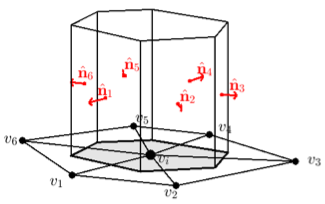
\includegraphics[width=0.3\linewidth]{Fig_masscontinuity.png}
  \caption{The Voronoi cell (grey) of a vertex serves as the control volume in the finite volume approach. Ice flows through the vertical faces of the volume, while the surface and basal mass balance add or remove ice from the top and bottom faces, respectively}
\end{figure}

The conservation law for a single Voronoi cell reads:

\begin{equation}
\frac{\partial \overline{H_i}}{\partial t} = \left[ \frac{-1}{A_i} \sum_{c=1}^n \int_{\partial_c} \left( \mathbf{u}_c H_c \cdot d\mathbf{\hat{n_c}} \right) \right] + \overline{M_i}.
\end{equation}

Here, the Voronoi cell of vertex $i$ shares the boundary $\partial_c$ with that of neighbouring vertex $c$. The equation is then discretised in space by assuming that the ice velocity $\textbf{u}$ and the ice thickness $H$ are constant on $\partial_c$, so that the line integral becomes a simple multiplication with the length $L_c$ of the shared boundary $\partial_c$:

\begin{equation}
\frac{\partial \overline{H_i}}{\partial t} = \left[ \frac{-1}{A_i} \sum_{c=1}^n \left( L_c \mathbf{u}_c H_c \cdot d\mathbf{\hat{n_c}} \right) \right] + \overline{M_i}.
\end{equation}

Lastly, the equation is discretised explicitly in time:

\begin{equation}
H_i^{t+\Delta t} = H_i^t + \Delta t \left( \left[ \frac{-1}{A_i} \sum_{c=1}^n \left( L_c \mathbf{u}_c H_c \cdot d\mathbf{\hat{n_c}} \right) \right] + \overline{M_i} \right).
\end{equation}

To calculate the ice fluxes, the ice velocities need to be known on the cell boundaries (i.e. the Arakawa C mesh). However, UFEMISM solves the SIA, the SSA, and/or the DIVA on the triangles (i.e. the Arakawa B mesh); velocities on the boundaries are calculated simply by averaging the values of the two adjacent triangles.

\newpage
\subsection{Time-stepping}

\subsubsection{Direct}

For the SIA, SSA, or hybrid SIA/SSA, "direct" time-stepping can be used. This makes use of the analytically-derived critical time steps for the SIA and SSA. For the SIA, this is the CFL-criterion:

\begin{equation} \label{eq:timestep_01}
\Delta t_{\textrm{SIA}} < \min \frac{\Delta^2}{6D}.
\end{equation}

For the SSA, this is the advective criterion:

\begin{equation} \label{eq:timestep_02}
\Delta t_{\textrm{SSA}} < \min \frac{\Delta}{|u| + |v|}.
\end{equation}

When the hybrid SIA/SSA is used, the models solve these two equatiosn asynchronously, each using its own time step. Since generally $\Delta t_{\textrm{SIA}} << \Delta t_{\textrm{SSA}}$, but solving the SSA is much more computationally expensive, this asynchronous approach is much more computationally efficient than a simpler synchronous scheme.

\subsubsection{Predictor/corrector}

By default, the models use a predictor/corrector time-stepping scheme. This scheme can be applied to any stress balance approximation; for the DIVA, it is currently the only available option. The implementation in IMAU-ICE and UFEMISM is largely adopted from Yelmo (Robinson et al., 2020).\\
\\
Each time step consists of three parts:

\begin{itemize}
\item \textit{Predictor step}: The ice thickness equation is solved using the \textit{current} ice thickness and velocity solution.
\item \textit{Update step}: A new velocity solution is calculated using the \textit{predicted} ice thickness.
\item \textit{Corrector step}: The ice thickness equation is solved again, using the \textit{current} ice thickness and the \textit{new} velocity solution.
\end{itemize}

The equation for the predictor step reads:

\begin{equation} \label{eq:timestep_03}
H_{n+1}^{\star} = H_n + \Delta t_n \left[ { 
\left( 1 + \frac{\zeta_t}{2} \right) \frac{\partial H}{\partial t} \left( H_n, \overline{\textbf{u}}_n \right)
- \frac{\zeta_t}{2} \frac{\partial H}{\partial t} \left( H_{n-1}, \overline{\textbf{u}}_{n-1} \right) } \right].
\end{equation}

Here, $\zeta_t$ is the ratio of the current over the previous time step:

\begin{equation} \label{eq:timestep_04}
\zeta_t = \frac{\Delta t_n}{\Delta t_{n-1}}.
\end{equation}

In the update step, the new ice velocities $\overline{\textbf{u}}_{n+1}$ are then calculated using the predicted ice geometry $H_{n+1}^{\star}$. The equation for the corrector step then reads:

\begin{equation} \label{eq:timestep_05}
H_{n+1} = H_n + \frac{\Delta t_n}{2} \left[ 
\frac{\partial H}{\partial t} \left( H_n, \overline{\textbf{u}}_n \right) +
\frac{\partial H}{\partial t} \left( H_{n+1}^{\star}, \overline{\textbf{u}}_{n+1} \right)
\right].
\end{equation}

The next time step $\Delta t_{n+1}$ is calculated by adapting the current time step $\Delta t$ based on the estimated truncation error $\tau$:

\begin{align} \label{eq:timestep_06}
\tau_{n+1} &= \frac{\zeta_t \left( H_{n+1} - H_{n+1}^{\star} \right) }{\left( 3 \zeta_t + 3 \right) \Delta t_n}, \\
\eta &= \max \left| \tau \right|, \\
\Delta t_{n+1} &= {\left( \frac{\epsilon}{\eta_{n+1}} \right)}^{k_I + k_p}
{\left( \frac{\epsilon}{\eta_n} \right) }^{-k_p} \Delta t_n.
\end{align}

The values for the control parameters $k_I = \frac{2}{10}$, $k_p = \frac{1}{10}$ are adopted from Yelmo.

\newpage
\subsection{Sliding}

Different sliding laws can be used to calculate the basal friction coefficient $\beta_b$ in the SSA/DIVA. Note that the Coulomb, regularised Coulomb, and Zoet-Iverson laws all express bed roughness in terms of the till friction angle $\phi$; the Weertman law uses $\beta^2$; and the Tsai2015 and Schoof2005 laws use both $\beta^2$ and $\alpha^2$. This means the user must take care to use an appropriate combination of sliding law and bed roughness formulation, as not all combinations are valid (e.g. the Martin2011 bed roughness parameterisation calculates $\phi$, but not $\beta^2$ or $\alpha^2$).

\subsubsection{Sliding laws}

\paragraph{Weertman}
The formulation of the Weertman-type (power law) sliding law used in IMAU-ICE and UFEMISM is based on that by Asay-Davis et al. (2016):

\begin{equation} \label{eq:slid_Weertman}
\beta_b = \beta^2 u_B^{\frac{1}{m}-1}.
\end{equation}

By default, $m=3$ (configurable); since the Weertman law describes the ice itself viscously deforming around large, immovable obstructions, it is advisable to let $m=n$, with $n$ the exponent in Glen's flow law.

\paragraph{Coulomb}
The Coulomb-type sliding law relates the basal friction coefficient to the effective overburden pressure $N = \rho_i g H - p_w$, and the till friction angle $\phi$:

\begin{equation} \label{eq:slid_Coulomb}
\beta_b = N \tan \phi u_b^{-1}.
\end{equation}

\paragraph{regularised Coulomb}
The "regularised Coulomb" sliding law is adopted from PISM (Martin et al., 2011), which is in turn based on the formulation by Bueler and van Pelt (2015):

\begin{equation} \label{eq:slid_Coulomb_reg}
\beta_b = N \tan \phi \frac{u_b^{q-1}}{u_0^q}.
\end{equation}

By default, $u_0 = 100$ m/yr, and $q=0.3$.

\paragraph{Tsai 2015}
The formulation of the hybrid sliding law by Tsai et al. (2015) is adopted from Asay-Davis et al. (2016):

\begin{equation} \label{eq:slid_Tsai2015}
\beta_b = \min \left( \alpha^2 N, \beta^2 u_b^{\frac{1}{m}}\right) u_b^{-1}.
\end{equation}

The Coulomb friction parameter $\alpha^2$ appearing here and in the Schoof2005 law is essentially identical to $\tan \phi$ in the Coulomb, regularised Coulomb, and Zoet-Iverson laws.

\paragraph{Schoof 2005}
The formulation of the hybrid sliding law by Schoof (2005) is adopted from Asay-Davis et al. (2016):

\begin{equation} \label{eq:slid_Schoof2005}
\beta_b = \frac{\beta^2 u_b^{\frac{1}{m}} \alpha^2 N }
{{\left[ \beta^{2m} u_b + {\alpha^2 N}^m \right]}^{\frac{1}{m}}} u_b^{-1}.
\end{equation}

The Coulomb friction parameter $\alpha^2$ appearing here and in the Tsai2015 law is essentially identical to $\tan \phi$ in the Coulomb, regularised Coulomb, and Zoet-Iverson laws.

\paragraph{Zoet-Iverson}
The sliding law formulated by Zoet and Iverson (2020) is expressed as:

\begin{equation} \label{eq:slid_ZoetIverson}
\beta_b = N \tan \phi \frac{ u_b^{ \frac{1}{p}-1} } { {\left( u_b + u_t \right) }^{\frac{1}{p}} }
\end{equation}

By default, $u_t = 200$ m/yr, and $p = 5$.

\paragraph{Idealised options}
Some of the ISMIP-HOM experiments use expressions for $\beta_b$ that are not dependent on $u_b$. These special cases can be selected by setting \textsc{choice\textunderscore sliding\textunderscore law} to \textsc{'idealised'}, and choosing the desired option using \textsc{choice\textunderscore idealised\textunderscore sliding\textunderscore law}.

\subsubsection{Sub-grid friction scaling}

Both IMAU-ICE and UFEMISM achieve good grounding-line migration (with relatively little hysteresis or dependence on grid resolution) by using a sub-grid friction scaling scheme, similar to PISM (Feldmann et al., 2014) and CISM (Leguy et al., 2021). This has replaced the grounding-line flux condition that was included in UFEMISM v1.0 (Berends et al., 2021). The sub-grid friction scheme offers greatly improved numerical stability over the flux condition, as well as far easier implementation, without requiring a long list of exceptions for different geometrical settings, as was the case for the flux condition.\\
\\
IMAU-ICE adopts the approach from CISM, where, within each quarter grid cell, the grounded fraction is calculated using the analytical solution to the bilinear interpolation equation provided by Leguy et al. (2021). Quarter grid cells are used so that the grounded fraction can be calculated on all four Arakawa grids (A, B, Cx, and Cy) without loss of accuracy. The basal friction coefficient $\beta_b$ is multiplied with the square of the grounded fraction. This is a small deviation from CISM and PISM, which don't use the square. However, PISM also uses a one-sided differencing scheme to calculate the driving stress near the grounding line, made possible by the fact that they calculate the ice velocities on the regular Arakawa A-grid instead of the staggered Arakawa C-grid. This likely introduces a second order of dependence on the ice thickness, which we create by using the square of the grounded fraction. CISM does neither, but calculates the velocity on the Arakawa B-grid, which might also affect the behaviour of the solution.\\
\\
UFEMISM follows the same general approach. However, the calculation of the grounded fractions is made simpler because of the triangular grid (a rare occasion indeed!), so that we need only solve the equation for trilinear instead of bilinear interpolation.

\subsubsection{Bed roughness}

The calculation of the bed roughness can be chosen independent of the sliding law.

\paragraph{Uniform}
The simplest option is to use a spatially and temporally uniform bed roughness.

\paragraph{Martin 2011}
For the sliding laws that express bed roughness in terms of the till friction angle $\phi$ (Coulomb, regularised Coulomb, and Zoet-Iverson), the bedrock elevation-dependent parameterisation by Martin et al. (2011) can be used:

\begin{align} \label{eq:slid_bedroughness_01}
\phi &= w_b \phi_{\textrm{max}} + \left( 1 - w_b \right) \phi_{\textrm{min}}, \\
w_b &= \min \left( 1, \max \left( 0, \frac{ b - b_{\textrm{min}} } { b_{\textrm{max}} - b_{\textrm{min}} } \right) \right).
\end{align}

By default, $\phi_{\textrm{min}} = 5 \degree$, $\phi_{\textrm{max}} = 20 \degree$, $b_{\textrm{min}} = -1000$ m, and $b_{\textrm{max}} = 0$ m. The Martin2011 bed roughness parameterisation can be selected by setting \textsc{choice\textunderscore basal\textunderscore roughness} to \textsc{'parameterised'}, and \textsc{choice\textunderscore param\textunderscore basal\textunderscore roughness} to \textsc{'Martin2011'}.

\paragraph{Idealised options}
For the SSA ice stream experiment, and some of the schematic basal inversion experiments, several unique parameterisations for the bed roughness are available. These special cases can be selected by setting \textsc{choice\textunderscore basal\textunderscore roughness} to \textsc{'parameterised'}, and choosing the desired option using \textsc{choice\textunderscore param\textunderscore basal\textunderscore roughness}.

\subsubsection{Basal hydrology}

The basal hydrology module calculates the pore water pressure in the subglacial till, which affects the effective overburden pressure in the calculation of the basal friction coefficients in the Coulomb, regularised Coulomb, and Zoet-Iverson sliding laws. Currently, only two very simple basal hydrology models are included: "saturated", and "Martin2011". This is one of the bigger weaknesses of the two models, and needs to be addressed in future work.

\paragraph{Saturated}
In the saturated till model, the pore water pressure is always equal to the hydrostatic water pressure, i.e. assuming perfect ocean connectivity everywhere:

\begin{equation} \label{eq:slid_hydro_01}
p_w = -\rho_w g \left( SL - b \right)
\end{equation}

\paragraph{Martin2011}
In the Martin2011 till model, adopted from PISM (Martin et al., 2011), the pore water pressure depends on the ice thickness:

\begin{align} \label{eq:slid_hydro_02}
p_w &= 0.96 \rho_i g H \lambda_w, \\
\lambda_w &= min \left( 1, \max \left( 0, \frac{SL - b}{d_{\textrm{sat}} } \right) \right).
\end{align}

By default, $d_{\textrm{sat}} = 1000$ m.

\subsection{Calving}

Right now, the only available calving law is a simple threshold-thickness law, with a default threshold value \textsc{calving\textunderscore threshold\textunderscore thickness} = 200 m. Some additional calving-related options are:

\begin{itemize}
\item \textsc{do\textunderscore remove\textunderscore shelves} Remove all floating ice. Used e.g. in the ABUMIP-ABUK experiment.
\item \textsc{remove\textunderscore shelves\textunderscore larger\textunderscore than\textunderscore PD} Remove all ice in areas that are ice-free at present day.
\item \textsc{continental\textunderscore shelf\textunderscore calving} Remove all floating ice in ocean cells with a water depth greater than \textsc{continental\textunderscore shelf\textunderscore min\textunderscore height}.
\end{itemize}

\newpage
\section{Thermodynamics}

\subsection{Heat equation}

\textit{Copy the derivation of the discretisation from the old documentation.}

\subsection{Geothermal heat flux}

\textit{Uniform or from a provided external file.}

\newpage
\section{Climate}

\textit{Temperature and precipitation.}

\subsection{Matrix method}

\subsubsection{Temperature}

\subsubsection{Precipitation}

\subsection{Idealised options}

\newpage
\section{Ocean}

\textit{Temperature and salinity.}

\subsection{Matrix method}

\subsection{Shelf cavity extrapolation}

\subsection{Idealised options}

\newpage
\section{Surface mass balance}

\subsection{IMAU-ITM}

\subsection{Idealised options}

\newpage
\section{Basal mass balance}

\textit{Here we have a number of options, very nice!}

\subsection{Local parameterisations}

\textit{The three Favier2019 parameterisations.}

\subsection{PICO}

\subsection{Plume model}

\subsection{PICOP}

\subsection{Idealised options}

\newpage
\section{GIA}

\textit{In the far and distant past, roughly forty million years,\\
Antarctica was a lovely place with beaches and blue sky.\\
But a drop in atmospheric CO2 did then occur,\\
and now the continent is covered by an ice sheet three miles high.\\
\\
The Earth's crust has a hard time pushing back at all that ice;\\
it deforms in an elastic way (that's Hooke's low, don't you know!).\\
Underneath there's the asthenosphere, a layer of viscous rock,\\
which reacts on longer timescales, causing GLACIAL ISOSTATIC ADJUSTMENT!}

\subsection{ELRA}

\textit{Elastic Lithopshere, viscously Relaxing Asthenosphere}

\subsection{SELEN}

\textit{Gooo Paolo!}

\newpage
\section{Isotopes}

\textit{Do we say anything about the ANICE legacy model here?}

\newpage
\section{Forcing}

\subsection{Direct CO2}

\textit{Just read ice-core data from a text file.}

\subsection{Inverse method}

\textit{Dig up equations from Berends et al. 2019 for this part.}

\subsubsection{Global temperature offset}

\subsubsection{Atmospheric CO2}

\newpage
\part{Discretisation}

\section{IMAU-ICE}

\subsection{Arakawa grids}

IMAU-ICE uses a regular square grid to discretise the equations. Following standard practice in ice-sheet models, a staggered grid is used to solve the velocity equations. Scalar quantities (ice thickness, temperature, viscosity, etc.) are defined on the regular (Arakawa A) grid, whereas vector quantities (surface slopes, velocities) are defined on the staggered Arakawa C grids. These are depicted in Fig. X.

\begin{figure}[H]
  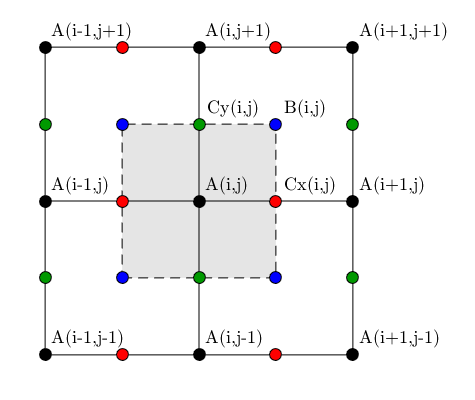
\includegraphics[width=0.5\linewidth]{Fig_IMAUICE_grids.png}
  \caption{The Arakawa grids used in IMAU-ICE: regular (A; black), x-staggered (Cx; red), y-staggered (Cy; green), and double-staggered (B; blue). A single grid cell is outlined in the centre.}
\end{figure}

Wherever the distinction between the Arakawa grids is relevant, data fields in the model have an extension in their name indicating on which grid the field is defined, e.g. \textsc{Hi\textunderscore a} is the ice thickness on the a-grid, and \textsc{Hi\textunderscore cx} is the ice thickness on the cx-grid. Note that these arrays will be of different sizes; \textsc{Hi\textunderscore a} is of size [$n_x$-by-$n_y$], whereas \textsc{Hi\textunderscore cx} is of size [$\left( n_x - 1 \right)$-by-$n_y$].

\subsection{Discretising the DIVA}

Consider the first equation of the DIVA stress balance (explained in more detail in Chapter X), where $N = \overline{\eta} H$:

\begin{equation}\label{eq:DIVA_disc_01}
\frac{\partial}{\partial x} \left[ 2 N \left( 2 \frac{\partial \overline{u}}{\partial x} + 
\frac{\partial \overline{v}}{\partial y} \right) \right] + 
\frac{\partial}{\partial y} \left[ N \left( \frac{\partial \overline{u}}{\partial y} + 
\frac{\partial \overline{v}}{\partial x} \right) \right] - \beta_{\textrm{eff}} \overline{u} = -\tau_{d,x}.
\end{equation}

Being a vector quantity, the x-velocity $u$ is defined on the cx-grid. We first discretise the gradient operators outside the square brackets, which yields:

\begin{equation} \label{eq:DIVA_disc_02}
\begin{split}
\frac{ { \left[ 2 N \left( 2 \frac{\partial \overline{u} }{\partial x} +
\frac{\partial \overline{v}}{\partial y} \right) \right] }_a^{i+1,j} }{\Delta} &-
\frac{ { \left[ 2 N \left( 2 \frac{\partial \overline{u} }{\partial x} +
\frac{\partial \overline{v}}{\partial y} \right) \right] }_a^{i,j} }{\Delta} + \\
\frac{ { \left[ N \left( \frac{\partial \overline{u} }{\partial y} +
\frac{\partial \overline{v}}{\partial x} \right) \right] }_b^{i,j} }{\Delta} &-
\frac{ { \left[ N \left( \frac{\partial \overline{u} }{\partial y} +
\frac{\partial \overline{v}}{\partial x} \right) \right] }_b^{i,j-1} }{\Delta}
- \beta_{\textrm{eff},cx}^{i,j} \overline{u}_{cx}^{i,j} = -\tau_{d,x,cx}^{i,j}.
\end{split}
\end{equation}

The derivatives of $u$,$v$ inside the square brackets can then also be discretised, leading :

\begin{equation} \label{eq:DIVA_disc_03}
\begin{split}
\frac{ 2 N_a^{i+1,j}}{\Delta^2} & \left( 2 \overline{u}_{cx}^{i+1,j} - 2 \overline{u}_{cx}^{i,j} +
\overline{v}_{cy}^{i+1,j} - \overline{v}_{cy}^{i+1,j-1} \right) - \\
\frac{ 2 N_a^{i,j}}{\Delta^2} & \left( 2 \overline{u}_{cx}^{i,j} - 2 \overline{u}_{cx}^{i-1,j} +
\overline{v}_{cy}^{i,j} - \overline{v}_{cy}^{i,j-1} \right) + \\
\frac{ N_b^{i,j}}{\Delta^2} & \left( \overline{u}_{cx}^{i,j+1} - \overline{u}_{cx}^{i,j} +
\overline{v}_{cy}^{i+1,j} - \overline{v}_{cy}^{i,j} \right) - \\
\frac{ N_b^{i,j-1}}{\Delta^2} & \left( \overline{u}_{cx}^{i,j} - \overline{u}_{cx}^{i,j-1} +
\overline{v}_{cy}^{i+1,j-1} - \overline{v}_{cy}^{i,j-1} \right)
- \beta_{\textrm{eff},cx}^{i,j} \overline{u}_{cx}^{i,j} = -\tau_{d,x,cx}^{i,j}.
\end{split}
\end{equation}

This system of linear equations can be represented by a matrix equation, where the matrix contains 9 non-zero elements per row, which can be solved using any preferred method.\\
\\
The horizontal strain rates $\frac{\partial \overline{u}}{\partial x}$, $\frac{\partial \overline{u}}{\partial y}$, $\frac{\partial \overline{v}}{\partial x}$, $\frac{\partial \overline{v}}{\partial y}$, the effective strain rate $\dot{\epsilon}_e$, the effective viscosity $\overline{\eta}$, and the product term $N$, are all calculated on the a-grid; $N_b$ is obtain by staggering $N_a$. The vertical shear strain rates $\frac{\partial u(z)}{\partial z}$, $\frac{\partial v(z)}{\partial z}$ are calculated on the cx/cy-grids, and then unstaggered to the a-grid. The sliding/vertical shear term $\beta_{\textrm{eff}}$ is calculated on the a-grid, and then staggered to the cx/cy-grids, where it is scaled with the sub-grid grounded fractions (which are calculated directly on those grids to preserve accuracy).

\newpage
\section{UFEMISM}

\subsection{Mesh}

\subsubsection{Nomenclature}

Consider the simple mesh shown in Fig. \ref{fig:dummymesh}.

\begin{figure}[h!] \label{fig:dummymesh}
  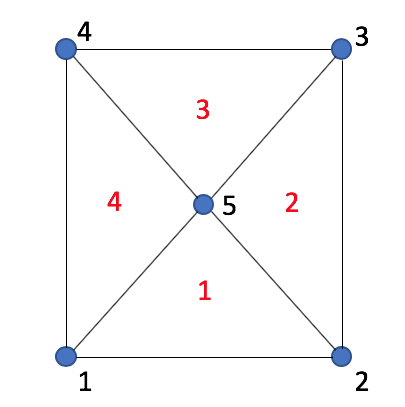
\includegraphics[width=0.3\linewidth]{Fig_dummymesh_02.png}
  \caption{A simple mesh.}
\end{figure}

This \emph{mesh} consists of five \emph{vertices}, each connected to several others by \emph{lines} and/or \emph{segments}, which together span four \emph{triangles}. A connection between two vertices is called a line when the connection is a shared border of two triangles. Connections that are part of the domain boundary (and thus form the border of only a single triangle) are called segments. Vertices 1 and 2 are connected by a segment, vertices 1 and 5 are connected by a line.

\subsubsection{Voronoi cells and Delaunay triangulation}

A \emph{triangulation} is a way to connect a given set of points in $\mathbb{R}^{2}$, such that each point is connected to at least two others by lines spanning triangles (and nothing else), without any intersecting lines. There generally exist many different triangulations for any set of points, but there is always a single unique one, called the \emph{Delaunay triangulation}, which exhibits several useful properties. Formally, the Delaunay triangulation is defined as the triangulation where the circumcircle of any triangle contains does not contain any points inside it other than the three points spanning the triangle. However, this definition is not very easy to comprehend. Instead, it is more intuitive to define the Delaunay triangulation using the concept of Voronoi cells.\\
\\
For a given set of points in $\mathbb{R}^{2}$, each point can be assigned a region of space that is closer to that point than to any other point. This region is called the \emph{Voronoi cell} belonging to that point. The Delaunay triangulation is the triangulation where a point is connected to another point if and only if their Voronoi cells share a boundary. This is illustrated in Fig. \ref{fig:VoronoiDelaunay}.

\begin{figure}[h!] \label{fig:VoronoiDelaunay}
  \centering
  \begin{subfigure}[b]{0.25\linewidth}
    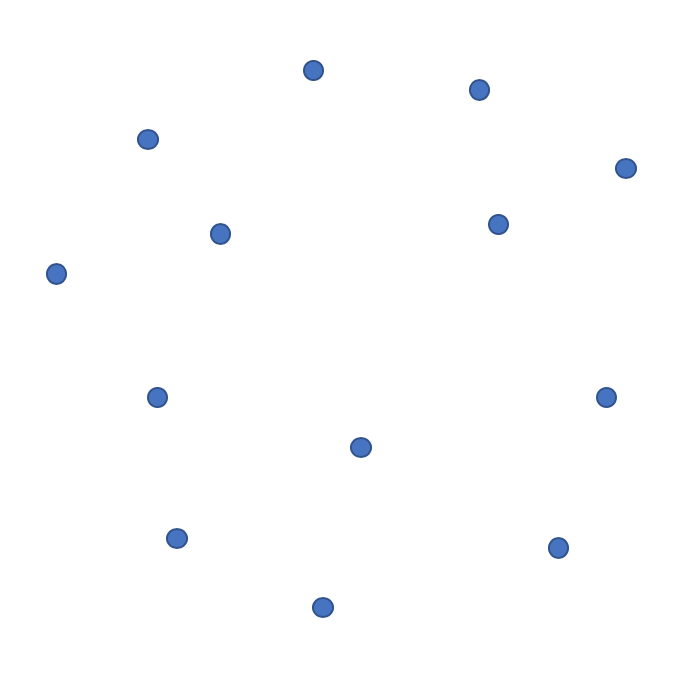
\includegraphics[width=\linewidth]{Fig_VoronoiDelaunay_01.png}
    \caption{}
  \end{subfigure}
  \begin{subfigure}[b]{0.25\linewidth}
    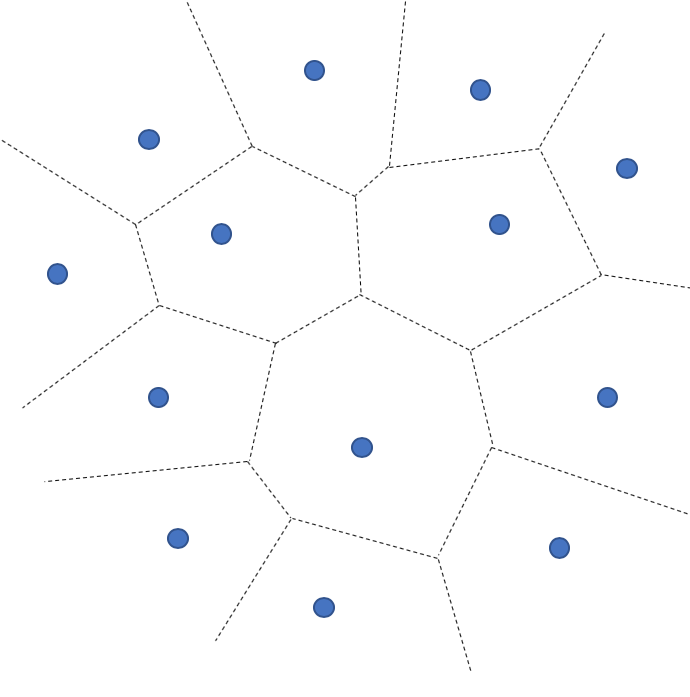
\includegraphics[width=\linewidth]{Fig_VoronoiDelaunay_02.png}
    \caption{}
  \end{subfigure}
  \begin{subfigure}[b]{0.25\linewidth}
    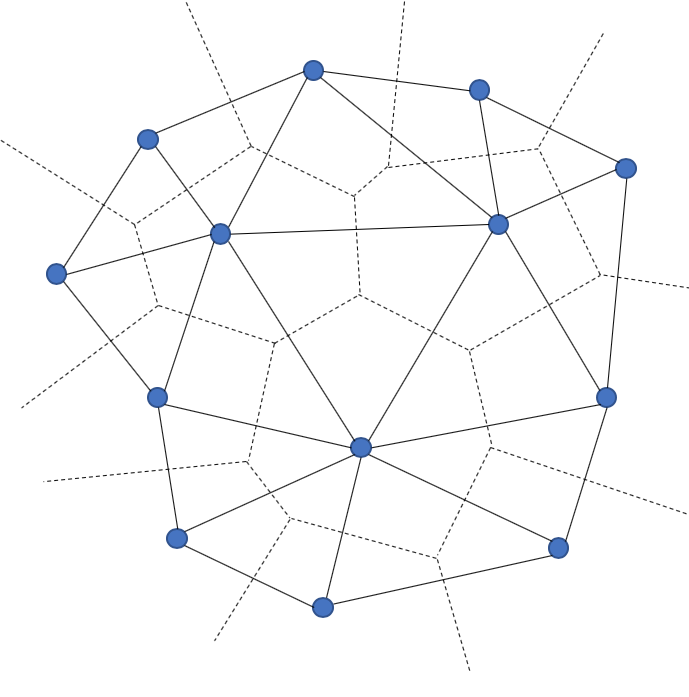
\includegraphics[width=\linewidth]{Fig_VoronoiDelaunay_03.png}
    \caption{}
  \end{subfigure}
  \caption{(a) A collection of points in $\mathbb{R}^{2}$, (b) the Voronoi cells of the points, (c) the Delaunay triangulation.}
\end{figure}

While we will not prove them, some useful properties of the Delaunay triangulation are:

\begin{itemize}
  \item The line connecting two points is always perpendicular to the shared boundary of their respective Voronoi cells.
  \item The Delaunay triangulation minimises the smallest internal angle of all triangles.
\end{itemize}

These two properties are especially useful in the context of ice-sheet models (and other fluid dynamics models). The first property is very useful when using a finite volume approach to solve the mass conservation equation, while the second one is useful for improving numerical stability. As far as I've been able to find, all models that use unstructured triangular grids use the Delaunay triangulation.\\
\\
It can be proven mathematically (if one were of a mind to do so) that any triangulation can be changed into the Delaunay triangulation by iteratively finding triangle pairs that violate the local Delaunay criterion (i.e. where the fourth vertex lies inside the circumcircle of the other three), and "flipping" them. This is illustrated in Fig. \ref{fig:Delaunayflip}.

\begin{figure}[h!] \label{fig:Delaunayflip}
  \centering
  \begin{subfigure}[b]{0.3\linewidth}
    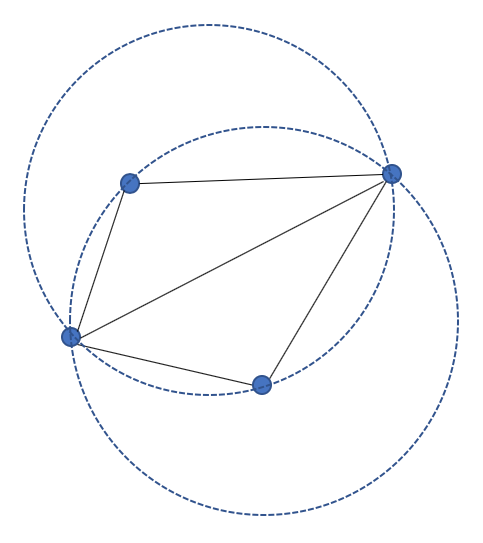
\includegraphics[width=\linewidth]{Fig_Delaunayflip_01.png}
    \caption{}
  \end{subfigure}
  \begin{subfigure}[b]{0.3\linewidth}
    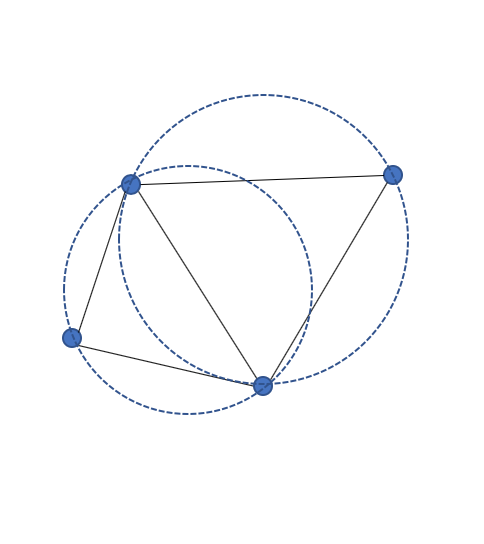
\includegraphics[width=\linewidth]{Fig_Delaunayflip_02.png}
    \caption{}
  \end{subfigure}
  \caption{(a) This pair of triangles violates the local Delaunay criterion, (b) the pair has been "flipped", and now satisfies the criterion.}
\end{figure}

\subsubsection{Data structure}

Theoretically, all that is needed to uniquely and completely describe a mesh is a list of the coordinates of its vertices. Everything else flows from there; their position in space determines the geometry of their Voronoi cells, which determines the Delaunay triangulation, which determines the connectivity. However, deriving all this information from the vertex coordinates can be a lengthy process, so instead several different forms of the mesh connectivity are stored in memory as well.\\
\\
A mesh consisting of \textit{nV} vertices and \textit{nTri} triangles is stored in memory in the form of vertex data and triangle data:

\begin{table}[H] \label{tab:table_vertexdatademo}
  \begin{center}
    \caption{Vertex data}
    \begin{tabular}{l|l|l}
      \textbf{Name} & \textbf{Description} & \textbf{Size}\\
      \hline
      V & Vertex [x,y] coordinates & DOUBLE(nV,2)\\
      nC & Number of connected vertices & INT(nV) \\
      C & Indices of connected vertices & INT(nV,32) \\
      niTri & Number of triangles containing this vertex & INT(nV) \\
      iTri & Indices of triangles containing this vertex & INT(nV,32) \\
      edge\textunderscore index & Edge index & INT(nV)\\
    \end{tabular}
  \end{center}
\end{table}

\begin{table}[H] \label{tab:table_triangledatademo}
  \begin{center}
    \caption{triangle data}
    \begin{tabular}{l|l|l}
      \textbf{Name} & \textbf{Description} & \textbf{Size}\\
      \hline
      Tri & Indices of the three vertices spanning this triangle & INT(nTri,3)\\
      Tricc & [x,y] coordinates of the triangle's circumcentre & DOUBLE(nTri,2) \\
      TriC & Indices of connected triangles & INT(nTri,3) \\
      Tri\textunderscore edge\textunderscore index & Edge index & INT(nTri)\\
    \end{tabular}
  \end{center}
\end{table}

As the name "unstructured mesh" suggests, there is no particular order to the indices of the vertices or triangles, and no relation between their
indices and their position. However, the following rules apply:

\begin{itemize}
  \item \textbf{C}: neighbouring vertices are listed in counterclockwise order, and only the first \textit{nC}
   entries of the 32 values per vertex are used; all other entries are zero. For vertices lying on the domain boundary, the list may not "jump" outside the domain; if, for example, this vertex lies on the eastern border, the first entry must be the neighbour lying north of the vertex on the boundary, and the last one must be the neighbour lying south of the vertex on the boundary.
  \item \textbf{iTri}: triangles containing the vertex are listed in counterclockwise order, and only the first \textit{niTri}
   entries of the 32 values per vertex are used; all other entries are zero. For boundary vertices, the same rule applies as for \textbf{C}.
  \item \textbf{Tri}: the three vertices spanning a triangle are listed in counterclockwise order. There are no rules for which vertex is listed first, but it must correspond to the entries in \textbf{TriC}.
  \item \textbf{TriC}: the three neighbouring triangles are sorted such that the first neighbouring triangles lies opposite of the first vertex, the second one across from the second vertex, etc. If no neighbouring triangle exists (i.e. when this side of the triangle is part of the domain boundary), a zero is listed.
  \item \textbf{edge\textunderscore index}: the edge index describes if a vertex lies on the domain boundary: 1 = northern boundary, 2 = north-east corner, 3 = eastern boundary, etc., 0 = not on any boundary.
  \item \textbf{Tri\textunderscore edge\textunderscore index}: similar to the edge index of vertices. The corner values (2,4,6,8) are used when a triangle is
   situated such that two if its sides lie on different parts of the domain boundary.
\end{itemize}

We will illustrate these variables with an example. Consider the simple mesh shown in Fig. \ref{fig:meshdata_02}.

\begin{figure}[H] \label{fig:meshdata_02}
  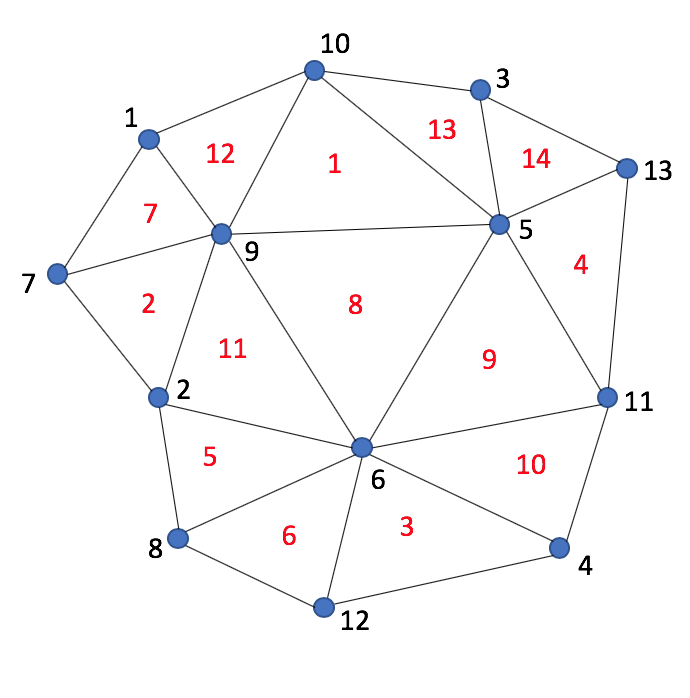
\includegraphics[width=0.5\linewidth]{Fig_meshdata_02.png}
  \caption{Another simple mesh.}
\end{figure}

The mesh data for this mesh is shown in Tables \ref{tab:table_vertexdata_01} and \ref{tab:table_triangledata_01}. Vertex coordinates \textbf{V} and triangle circumcentre coordinates \textbf{Tricc} are omitted for brevity.

\begin{table}[H] \label{tab:table_vertexdata_01}
  \begin{center}
    \caption{Vertex data}
    \begin{tabular}{l|l|l|l|l|l}
      \textbf{vi} & \textbf{V} & \textbf{nC} & \textbf{C} & \textbf{niTri} & \textbf{iTri}\\
      \hline
      1 & ... & 3 & 7,9,10 & 2 & 7,12\\
      2 & ... & 4 & 8,6,9,7 & 3 & 5,11,2\\
      3 & ... & 3 & 10,5,13 & 2 & 13,14\\
      4 & ... & 3 & 11,6,12 & 2 & 10,3\\
      5 & ... & 6 & 13,3,10,9,6,11 & 6 & 8,9,4,14,13,1\\
      6 & ... & 7 & 9,2,8,12,4,11,5 & 7 & 3,10,9,8,11,5,6\\
      7 & ... & 3 & 2,9,1 & 2 & 2,7\\
      8 & ... & 3 & 12,6,2 & 2 & 6,5\\
      9 & ... & 6 & 10,1,7,2,6,5 & 6 & 2,11,8,1,12,7\\
      10 & ... & 4 & 1,9,5,3 & 3 & 12,1,13\\
      11 & ... & 4 & 13,5,6,4 & 3 & 4,9,10\\
      12 & ... & 3 & 4,6,8 & 2 & 3,6\\
      13 & ... & 3 & 3,5,11 & 2 & 14,4\\
    \end{tabular}
  \end{center}
\end{table}

\begin{table}[H] \label{tab:table_triangledata_01}
  \begin{center}
    \caption{Triangle data}
    \begin{tabular}{l|l|l|l}
      \textbf{ti} & \textbf{Tri} & \textbf{Tricc} & \textbf{TriC}\\
      \hline
      1 & 9,5,10 & ... & 13,12,8\\
      2 & 9,7,2 & ... & 0,11,7\\
      3 & 12,4,6 & ... & 10,6,0\\
      4 & 13,5,11 & ... & 9,0,14\\
      5 & 2,8,6 & ... & 6,11,0\\
      6 & 12,6,8 & ... & 5,0,3\\
      7 & 7,9,1 & ... & 12,0,2\\\
      8 & 9,6,5 & ... & 9,1,11\\
      9 & 6,11,5 & ... & 4,8,10\\
      10 & 4,11,6 & ... & 9,3,0\\
      11 & 9,2,6 & ... & 5,8,2\\
      12 & 10,1,9 & ... & 7,1,0\\
      13 & 5,3,10 & ... & 0,1,14\\
      14 & 13,3,5 & ... & 13,4,0\\
    \end{tabular}
  \end{center}
\end{table}

\subsubsection{Arakawa C-mesh}

In order to apply the finite volume method, we need to define ice fluxes on the boundaries of the Voronoi cells of the vertices. This means we need a way to efficiently keep track of these boundaries. This is done by creating a "staggered mesh", which is conceptually very similar to the Arakawa C-grid used in square-grid models.

\begin{figure}[H] \label{fig:staggeredmesh}
  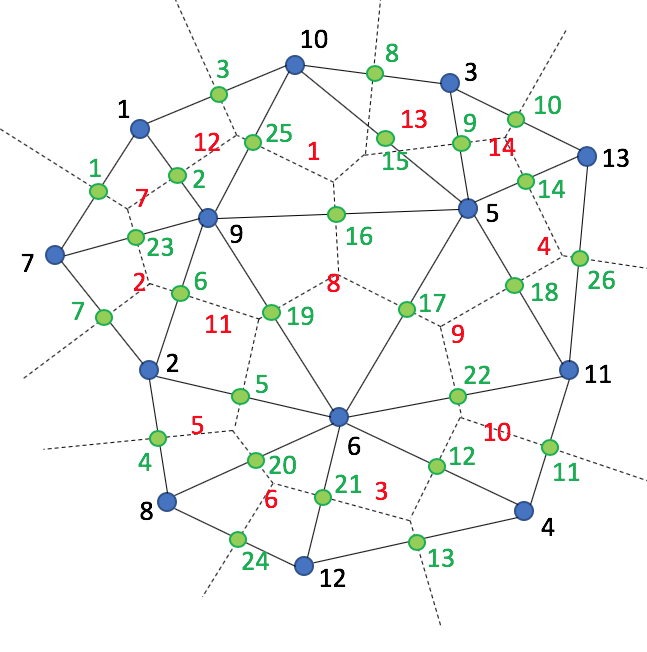
\includegraphics[width=0.5\linewidth]{Fig_staggeredmesh.png}
  \caption{The staggered vertices (green) correspond to the connections between the regular vertices (blue).}
\end{figure}

Each connection between two regular vertices is given a unique index, and represented by a staggered vertex lying halfway along the connection. Two lists are created, \textbf{Aci} and \textbf{iAci}, which relate regular vertices to staggered vertices, and vice versa. For the simple mesh shown above, these lists look like this:

\begin{table}[H] \label{tab:table_Acmesh}
  \begin{center}
    \begin{tabular}{l|l|l|l}
      \textbf{vi} & \textbf{iAci} & \textbf{ai} & \textbf{Aci}\\
      \hline
      1 & 1,2,3 & 1 & 1,7,9,0\\
      2 & 4,5,6,7 & 2 & 1,9,10,7\\
      3 & 8,9,10 & 3 & 1,10,0,9\\
      4 & 11,12,13 & 4 & 2,8,6,0\\
      5 & 14,9,15,16,17,18 & 5 & 2,6,9,8\\
      6 & 19,5,20,21,12,22,17 & 6 & 2,8,7,6\\
      7 & 7,23,1 & 7 & 2,7,0,9\\
      8 & 24,20,4 & 8 & 3,10,5,0\\
      9 & 25,2,23,6,19,16 & 9 & 3,5,13,10\\
      10 & 3,25,15,8 & 10 & 3,13,0,5\\
      11 & 26,18,22,11 & 11 & 4,11,6,0\\
      12 & 13,21,24 & 12 & 4,6,12,11\\
      13 & 10,14,26 & 13 & 4,12,0,6\\
      & & 14 & 5,13,3,11\\
      & & 15 & 5,10,9,3\\
      & & 16 & 5,9,6,10\\
      & & 17 & 5,6,11,9\\
      & & 18 & 5,11,13,6\\
      & & 19 & 6,9,2,5\\
      & & 20 & 6,8,12,2\\
      & & 21 & 6,12,4,8\\
      & & 22 & 6,11,5,4\\
      & & 23 & 7,9,1,2\\
      & & 24 & 8,12,6,0\\
      & & 25 & 9,10,1,5\\
      & & 26 & 11,13,5,0
    \end{tabular}
  \end{center}
\end{table}

\textbf{iAci} lists the staggered vertices surrounding each regular vertex. The ordering corresponds to that of \textbf{C}, so that the $j$'th staggered vertex listed for vertex $i$ lies halfway along the connection between $v_i$ and its $j$'th neighbour. \textbf{Aci} lists the regular vertices along whose connection each staggered vertex lies. Additionally, it lists the two regular vertices lying to the left and right of this connection, so that the four columns in a row of \textbf{Aci} read $[v_i,v_j,v_l,v_r]$, with $v_l$ lying to the left of the line from $v_i$ to $v_j$, and $v_r$ lying to the right. If either $v_l$ or $v_r$ does not exist (which can happen when $v_i$ and $v_j$ lie on the domain boundary), the entry is zero. Keeping track of $v_l$ and $v_r$ is very useful for calculating derivatives on the staggered vertices, as we will see in Sect. XXX on discretisation.\\

\newpage
\subsection{Discretisation}

Let $f: \mathbb{R}^{2} \rightarrow \mathbb{R}$ be a function defined on the model domain, and let $f_a$, $f_b$, $f_c$ be its discretised approximations on the mesh vertices, triangles, and edges, equivalent to the Arakawa A-, B-, and C-grids. For convenience, the discretised approximations to the partial derivatives of $f$ on the different grids are written as $f_{x,a} = {\left( \frac{\partial f}{\partial x} \right)}_a$, $f_{yy,c} = {\left( \frac{\partial^2 f}{\partial y^2} \right)}_c$, etc. These partial derivatives can be expressed as linear combinations of $f_a$, $f_b$, or $f_c$, e.g.:

\begin{equation} \label{eq:disc_mesh_01}
f_{x,a} = M_{x,a,a} f_a
\end{equation}

Here, $M_{x,a,a}$ is an $nV$-by-$nV$ matrix. In the notation convention used here, $M$ has three subscript letters. The first represents the operation: $x$ for $\frac{\partial}{\partial x}$, $y$ for $\frac{\partial}{\partial y}$, and $m$ for mapping. The second and third letters represent the source and destination grids, respectively (e.g. $M_{m,a,b}$ maps a data field from the vertices to the triangles).\\
\\
The coefficients in $M$ are called shape functions. They can be derived in different ways; UFEMISM uses the weighted least-squares approach described by Syrakos et al. (2017).

\subsubsection{First-order, regular grid}

Syrakos et al. (2017) describe a (weighted) least-squares approach to discretising the gradient operator on an unstructured triangular grid. Let $f_a^i$, $f_{x,a}^i$, $f_{y,a}^i$ be the values of the function $f$ and its first partial derivatives on vertex $i$. The value $f_a^j$ of $f$ on vertex $j$, which is connected to vertex $i$, can then be expressed as a Taylor expansion of $f$ around $i$: 

\begin{equation} \label{eq:disc_taylor}
f_a^j = f_a^i + \Delta x_j f_{x,a}^i + \Delta y_j f_{y,a}^i 
+ \mathcal{O} \left( \Delta x_j^2, \Delta y_j^2 \right).
\end{equation}

Here, $\Delta x_j$, $\Delta y_j$ is the horizontal displacement between $j$ and $i$. If $i$ has $n$ neighbours, this results in the following system of $n$ linear equations (defining $\Delta f_a^j \equiv f_a^j - f_a^i$, dropping the truncation error $\mathcal{O} \left( \Delta x_j^2, \Delta y_j^2 \right)$, and introducing the vertex weights $w_j$ for the weighted least-squares approximation:

\begin{equation} \label{eq:disc_LSmatrix}
\underbrace{\begin{bmatrix}
w_1 & 0 & \ldots & 0 \\ 0 & w_2 & \ldots & 0 \\ \vdots & \vdots & \ddots & \vdots \\ 0 & 0 & \ldots & w_n
 \end{bmatrix}}_W
\underbrace{\begin{bmatrix}
\Delta f_a^1 \\ \Delta f_a^2 \\ \vdots \\ \Delta f_a^n
 \end{bmatrix}}_b
 =
\underbrace{\begin{bmatrix}
w_1 & 0 & \ldots & 0 \\ 0 & w_2 & \ldots & 0 \\ \vdots & \vdots & \ddots & \vdots \\ 0 & 0 & \ldots & w_n
 \end{bmatrix}}_W
\underbrace{\begin{bmatrix}
\Delta x_1 & \Delta y_1 \\
\Delta x_2 & \Delta y_2 \\
\vdots & \vdots \\
\Delta x_n & \Delta y_n
 \end{bmatrix}}_A
\underbrace{\begin{bmatrix}
f_{x,a}^i \\ f_{y,a}^i
 \end{bmatrix}}_z.
\end{equation}

Using matrix notation, this equation reads $Wb = WAz$, which is solved for $z$ by writing:

\begin{equation} \label{eq:disc_LSmatrixz}
z = {\left( A^T W^T W A \right)}^{-1} A^T W^T W b = Q \beta_b.
\end{equation}

Here, we have grouped the $A$ and $W$ terms into $Q = {\left( A^T W^T W A \right)}^{-1}$ and $\beta_b = A^T W^T W b$. The symmetric matrix $A^T W^T W A$, which needs to be inverted to find $Q$, reads:

\begin{equation} \label{eq:disc_LSATWTWA}
A^T W^T W A = \sum_{c=1}^n w_c^2
\begin{bmatrix}
\Delta x_c^2 & \Delta x_c \Delta y_c \\
\Delta x_c \Delta y_c & \Delta y_c^2
\end{bmatrix}.
\end{equation}

The second term, $\beta_b$, is expressed as:

\begin{equation} \label{eq:disc_LSbetab}
\beta_b = \sum_{c=1}^n w_c^2
\begin{bmatrix}
\Delta x_c \Delta f_a^c \\ \Delta y_c \Delta f_a^c
\end{bmatrix}.
\end{equation}

Once $Q$ has been calculated by inverting $A^T W^T W A$, the first partial derivative $f_{x,a}^i$ of $f$ on $i$ can be expressed as:

\begin{equation} \label{eq:disc_LSfxifyi}
f_{x,a}^i = 
Q(1,1) \sum_{c=1}^n \left( w_c^2 \Delta x_c \Delta f_a^c \right) + 
Q(1,2) \sum_{c=1}^n \left( w_c^2 \Delta y_c \Delta f_a^c \right).
\end{equation}

Since $\Delta f_a^c = f_a^c - f_a^i$, this can be rewritten to read:

\begin{equation}
\begin{split}
f_{x,a}^i = -f_a^i & \sum_{c=1}^n \left[ w_c^2 \left( Q(1,1) \Delta x_c + Q(1,2) \Delta y_c \right) \right] + \\
& \sum_{c=1}^n f_a^c \left[ w_c^2 \left( Q(1,1) \Delta x_c + Q(1,2) \Delta y_c \right) \right].
\end{split}
\end{equation}

This means that the shape functions $M_{x,a,a}^{i,j}$ for the partial derivative $f_{x,a}$ are given by:

\begin{equation}
M_{x,a,a}^{i,j} = \left\{
\begin{array}{ c l }
-\sum_{j=1}^n w_j^2 \left[ Q(1,1) \Delta x_j + Q(1,2) \Delta y_j \right] & \textrm{if } i = j, \\
w_j^2 \left( Q(1,1) \Delta x_j + Q(1,2) \Delta y_j \right) & \textrm{if } j \textrm{ is connected to } i, \\
0 & \textrm{otherwise}.
\end{array}
\right.
\end{equation}

Similarly, the shape functions $M_{y,a,a}^{i,j}$ for $f_{y,a}$ are given by:

\begin{equation}
M_{y,a,a}^{i,j} = \left\{
\begin{array}{ c l }
-\sum_{j=1}^n w_j^2 \left[ Q(2,1) \Delta x_j + Q(2,2) \Delta y_j \right] & \textrm{if } i = j, \\
w_j^2 \left( Q(2,1) \Delta x_j + Q(2,2) \Delta y_j \right) & \textrm{if } j \textrm{ is connected to } i, \\
0 & \textrm{otherwise}.
\end{array}
\right.
\end{equation}

The weights $w_j$ depend on the distance between $j$ and $i$:

\begin{equation}
w_j = \frac{1}{ \left| \textbf{r}_j - \textbf{r}_i \right|^q}.
\end{equation}

Following Syrakos et al. (2017), $q = \frac32$.

\subsubsection{First-order, staggered grid}

The derivation in the previous section assumes that the grids where we know $f$ and where we want to know $f_x$, $f_y$ are the same. However, if for example we know $f_a$ and we want to know $f_{x,b}$ then this assumption does not hold, and the derivation of the shape functions looks slightly different.\\
\\
Consider once again the Taylor series given by \eqref{eq:disc_taylor}. We once again write out the system of equations for all neighbours of $i$, but this time we do not introduce $\Delta f$, so that we obtain the following expression:

\begin{equation} \label{eq:disc_LSmatrix2}
\underbrace{\begin{bmatrix}
w_1 & 0 & \ldots & 0 \\ 0 & w_2 & \ldots & 0 \\ \vdots & \vdots & \ddots & \vdots \\ 0 & 0 & \ldots & w_n
 \end{bmatrix}}_W
\underbrace{\begin{bmatrix}
f_a^1 \\ f_a^2 \\ \vdots \\ f_a^n
 \end{bmatrix}}_b
 =
\underbrace{\begin{bmatrix}
w_1 & 0 & \ldots & 0 \\ 0 & w_2 & \ldots & 0 \\ \vdots & \vdots & \ddots & \vdots \\ 0 & 0 & \ldots & w_n
 \end{bmatrix}}_W
\underbrace{\begin{bmatrix}
1 & \Delta x_1 & \Delta y_1 \\
1 & \Delta x_2 & \Delta y_2 \\
\vdots & \vdots \\
1 & \Delta x_n & \Delta y_n
 \end{bmatrix}}_A
\underbrace{\begin{bmatrix}
f_b^i \\ f_{x,b}^i \\ f_{y,b}^i
 \end{bmatrix}}_z.
\end{equation}

Following the same derivation as before, the matrix $A^T W^T W A$ that needs to be inverted to find $Q$ is now given by:

\begin{equation}
A^T W^T W A = \sum_{c=1}^n w_c^2 \begin{bmatrix}
1 & \Delta x_c & \Delta y_c \\
& \Delta x_c^2 & \Delta x_c \Delta y_c \\
& & \Delta y_c^2
\end{bmatrix}.
\end{equation}

Similarly, $\beta_b$ is now given by:

\begin{equation}
\beta_b = \sum_{c=1}^n w_c^2 \begin{bmatrix} f_a^c \\ \Delta x_c f_ a^c \\ \Delta y_c f_a^c \end{bmatrix}.
\end{equation}

This leads to the following expression for the shape functions $M_{m,a,b}^{i,j}$, $M_{x,a,b}^{i,j}$, $M_{y,a,b}^{i,j}$:

\begin{equation}
M_{m,a,b}^{i,j} = \left\{
\begin{array}{ c l }
-\sum_{j=1}^n w_j^2 \left[ Q(1,1) + Q(1,2) \Delta x_j + Q(1,3) \Delta y_j \right] & \textrm{if } i = j, \\
w_j^2 \left( Q(1,1) + Q(1,2) \Delta x_j + Q(1,3) \Delta y_j \right) & \textrm{if } j \textrm{ is connected to } i, \\
0 & \textrm{otherwise};
\end{array}
\right.
\end{equation}

\begin{equation}
M_{x,a,b}^{i,j} = \left\{
\begin{array}{ c l }
-\sum_{j=1}^n w_j^2 \left[ Q(2,1) + Q(2,2) \Delta x_j + Q(2,3) \Delta y_j \right] & \textrm{if } i = j, \\
w_j^2 \left( Q(2,1) + Q(2,2) \Delta x_j + Q(2,3) \Delta y_j \right) & \textrm{if } j \textrm{ is connected to } i, \\
0 & \textrm{otherwise};
\end{array}
\right.
\end{equation}

\begin{equation}
M_{y,a,b}^{i,j} = \left\{
\begin{array}{ c l }
-\sum_{j=1}^n w_j^2 \left[ Q(3,1) + Q(3,2) \Delta x_j + Q(3,3) \Delta y_j \right] & \textrm{if } i = j, \\
w_j^2 \left( Q(3,1) + Q(3,2) \Delta x_j + Q(3,3) \Delta y_j \right) & \textrm{if } j \textrm{ is connected to } i, \\
0 & \textrm{otherwise}.
\end{array}
\right.
\end{equation}

\subsubsection{Second-order, regular grid}

Here, we extend the discretisation scheme by Syrakos et al. (2017) to include the second partial derivatives $f_{xx}$, $f_{xy}$, $f_{yy}$. First, we extend the Taylor expansion of $f$ around $i$ to the second order:

\begin{equation} \label{eq:disc_taylor2}
f_a^j = f_a^i + \Delta x_j f_{x,a}^i + \Delta y_j f_{y,a}^i
+ \frac12 \Delta x_j^2 f_{xx,a}^i + \Delta x_j \Delta y_j f_{xy,a}^i + \frac12 \Delta y_j^2 f_{yy,a}^i
+ \mathcal{O} \left( \Delta x_j^3, \Delta y_j^3 \right).
\end{equation}

Writing out the system of linear equations for all neighbours of $i$ now yields the following expression:

\begin{equation} \label{eq:disc_LSmatrix3}
\underbrace{\begin{bmatrix}
w_1 & 0 & \ldots & 0 \\ 0 & w_2 & \ldots & 0 \\ \vdots & \vdots & \ddots & \vdots \\ 0 & 0 & \ldots & w_n
 \end{bmatrix}}_W
\underbrace{\begin{bmatrix}
\Delta f_a^1 \\ \Delta f_a^2 \\ \vdots \\ \Delta f_a^n
 \end{bmatrix}}_b
 =
\underbrace{\begin{bmatrix}
w_1 & 0 & \ldots & 0 \\ 0 & w_2 & \ldots & 0 \\ \vdots & \vdots & \ddots & \vdots \\ 0 & 0 & \ldots & w_n
 \end{bmatrix}}_W
\underbrace{\begin{bmatrix}
\Delta x_1 & \Delta y_1 & \frac12 \Delta x_1^2 & \Delta x_1 \Delta y_1 & \frac12 \Delta y_1^2 \\
\Delta x_2 & \Delta y_2 & \frac12 \Delta x_2^2 & \Delta x_2 \Delta y_2 & \frac12 \Delta y_2^2 \\
\vdots & \vdots \\
\Delta x_n & \Delta y_n & \frac12 \Delta x_n^2 & \Delta x_n \Delta y_n & \frac12 \Delta y_n^2 
 \end{bmatrix}}_A
\underbrace{\begin{bmatrix}
f_{x,a}^i \\ f_{y,a}^i \\ f_{xx,a}^i \\ f_{xy,a}^i \\ f_{yy,a}^i
 \end{bmatrix}}_z.
\end{equation}

The matrix $A^T W^T W A$ that needs to be inverted to find $Q$ is now given by:

\begin{equation} \label{eq:disc_LSATWTWA2}
A^T W^T W A = \sum_{c=1}^n w_c^2
\begin{bmatrix}
\Delta x_c^2 & \Delta x_c \Delta y_c & \frac12 \Delta x_c^3 & \Delta x_c^2 \Delta y_c & \frac12 \Delta x_c \Delta y_c^2 \\
 & \Delta y_c^2 & \frac12 \Delta x_c^2 \Delta y_c & \Delta x_c \Delta y_c^2 & \frac12 \Delta y_c^3 \\ 
 & & \frac14 \Delta x_c^4 & \frac12 \Delta x_c^3 \Delta y_c & \frac14 \Delta x_c^2 \Delta y_c^2 \\ 
 & & & \Delta x_c^2 \Delta y_c^2 & \frac12 \Delta x_c \Delta y_c^3 \\
 & & & & \frac14 \Delta y_c^4
\end{bmatrix}.
\end{equation}

Similarly, $\beta_b$ is now given by:

\begin{equation} \label{eq:disc_LSbetab3}
\beta_b = \sum_{c=1}^n w_c^2
\begin{bmatrix}
\Delta x_c \Delta f_a^c \\ \Delta y_c \Delta f_a^c \\ \frac12 \Delta x_c^2 \Delta f_a^c \\ \Delta x_c \Delta y_c \Delta f_a^c \\ \frac12 \Delta y_c^2 \Delta f_a^c
\end{bmatrix}.
\end{equation}

This leads to the following expressions for the shape functions $M_{x,a,a}^{i,j}$, $M_{y,a,a}^{i,j}$, $M_{xx,a,a}^{i,j}$, $M_{xy,a,a}^{i,j}$, and $M_{yy,a,a}^{i,j}$:

\begin{equation}
M_{x,a,a}^{i,j} = \left\{
\begin{array}{ c l }
-\sum_{j=1}^n w_j^2 \left[ Q(1,1) \Delta x_j + Q(1,2) \Delta y_j + \frac12 Q(1,3) \Delta x_j^2 + \frac14 Q(1,4) \Delta x_j \Delta y_j + \frac12 Q(1,5) \Delta y_j^2 \right] & \textrm{if } i = j, \\
w_j^2 \left( Q(1,1) \Delta x_j + Q(1,2) \Delta y_j + \frac12 Q(1,3) \Delta x_j^2 + \frac14 Q(1,4) \Delta x_j \Delta y_j + \frac12 Q(1,5) \Delta y_j^2 \right) & \textrm{if } j \textrm{ is connected to } i, \\
0 & \textrm{otherwise};
\end{array}
\right.
\end{equation}

\begin{equation}
M_{y,a,a}^{i,j} = \left\{
\begin{array}{ c l }
-\sum_{j=1}^n w_j^2 \left[ Q(2,1) \Delta x_j + Q(2,2) \Delta y_j + \frac12 Q(2,3) \Delta x_j^2 + \frac14 Q(2,4) \Delta x_j \Delta y_j + \frac12 Q(2,5) \Delta y_j^2 \right] & \textrm{if } i = j, \\
w_j^2 \left( Q(2,1) \Delta x_j + Q(2,2) \Delta y_j + \frac12 Q(2,3) \Delta x_j^2 + \frac14 Q(2,4) \Delta x_j \Delta y_j + \frac12 Q(2,5) \Delta y_j^2 \right) & \textrm{if } j \textrm{ is connected to } i, \\
0 & \textrm{otherwise};
\end{array}
\right.
\end{equation}

\begin{equation}
M_{xx,a,a}^{i,j} = \left\{
\begin{array}{ c l }
-\sum_{j=1}^n w_j^2 \left[ Q(3,1) \Delta x_j + Q(3,2) \Delta y_j + \frac12 Q(3,3) \Delta x_j^2 + \frac14 Q(3,4) \Delta x_j \Delta y_j + \frac12 Q(3,5) \Delta y_j^2 \right] & \textrm{if } i = j, \\
w_j^2 \left( Q(3,1) \Delta x_j + Q(3,2) \Delta y_j + \frac12 Q(3,3) \Delta x_j^2 + \frac14 Q(3,4) \Delta x_j \Delta y_j + \frac12 Q(3,5) \Delta y_j^2 \right) & \textrm{if } j \textrm{ is connected to } i, \\
0 & \textrm{otherwise};
\end{array}
\right.
\end{equation}

\begin{equation}
M_{xy,a,a}^{i,j} = \left\{
\begin{array}{ c l }
-\sum_{j=1}^n w_j^2 \left[ Q(4,1) \Delta x_j + Q(4,2) \Delta y_j + \frac12 Q(4,3) \Delta x_j^2 + \frac14 Q(4,4) \Delta x_j \Delta y_j + \frac12 Q(4,5) \Delta y_j^2 \right] & \textrm{if } i = j, \\
w_j^2 \left( Q(4,1) \Delta x_j + Q(4,2) \Delta y_j + \frac12 Q(4,3) \Delta x_j^2 + \frac14 Q(4,4) \Delta x_j \Delta y_j + \frac12 Q(4,5) \Delta y_j^2 \right) & \textrm{if } j \textrm{ is connected to } i, \\
0 & \textrm{otherwise};
\end{array}
\right.
\end{equation}

\begin{equation}
M_{yy,a,a}^{i,j} = \left\{
\begin{array}{ c l }
-\sum_{j=1}^n w_j^2 \left[ Q(5,1) \Delta x_j + Q(5,2) \Delta y_j + \frac12 Q(5,3) \Delta x_j^2 + \frac14 Q(5,4) \Delta x_j \Delta y_j + \frac12 Q(5,5) \Delta y_j^2 \right] & \textrm{if } i = j, \\
w_j^2 \left( Q(5,1) \Delta x_j + Q(5,2) \Delta y_j + \frac12 Q(5,3) \Delta x_j^2 + \frac14 Q(5,4) \Delta x_j \Delta y_j + \frac12 Q(5,5) \Delta y_j^2 \right) & \textrm{if } j \textrm{ is connected to } i, \\
0 & \textrm{otherwise};
\end{array}
\right.
\end{equation}

\newpage
\subsubsection{Discretising the DIVA}

Consider the first equation of the DIVA stress balance (explained in more detail in Chapter X), where $N = \overline{\eta} H$:

\begin{equation} \label{eq:DIVA_discmesh_01}
\frac{\partial}{\partial x} \left[ 2 N \left( 2 \frac{\partial \overline{u}}{\partial x} + 
\frac{\partial \overline{v}}{\partial y} \right) \right] + 
\frac{\partial}{\partial y} \left[ N \left( \frac{\partial \overline{u}}{\partial y} + 
\frac{\partial \overline{v}}{\partial x} \right) \right] - \beta_{\textrm{eff}} \overline{u} = -\tau_{d,x}.
\end{equation}

Applying the product rule to remove the brackets, and using subscript notation for derivatives (e.g. $\overline{u}_x = \frac{\partial \overline{u}}{\partial x}$), yields:

\begin{equation} \label{eq:DIVA_discmesh_02}
4 N \overline{u}_{xx} + 4 N_x \overline{u}_x + 2 N \overline{v}_{xy} + 2 N_x \overline{v}_y +
N \overline{u}_{yy} + N_y \overline{u}_y + N \overline{v}_{xy} + N_y \overline{v}_x
- \beta_{\textrm{eff}} \overline{u} = -\tau_{d,x}.
\end{equation}

In UFEMISM, scalar quantities (ice thickness, temperature, viscosity, etc.) are defined on the a-grid (vertices), whereas velocities are defined on the b-grid (triangles). We discretise \eqref{eq:DIVA_discmesh_02} using the shape functions $M_{xx,b,b}$, $M_{yy,b,b}$, etc.:

\begin{equation} \label{eq:DIVA_discmesh_03}
\begin{split}
4 N_b M_{xx,b,b} \overline{u}_b &+ 4 N_{x,b} M_{x,b,b} \overline{u}_b +
2 N_b M_{xy,b,b} \overline{v}_b + 2 N_{x,b} M_{y,b,b} \overline{v}_b + \\
N_b M_{yy,b,b} \overline{u}_b &+ N_{y,b} M_{y,b,b} \overline{u}_b +
N_b M_{xy,b,b} \overline{v}_b + N_{y,b} M_{x,b,b} \overline{v}_b
- \beta_{\textrm{eff},b} \overline{u}_b = -\tau_{d,x,b}.
\end{split}
\end{equation}

Grouping together all terms including $\overline{u}$ and $\overline{v}$ yields:

\begin{equation} \label{eq:DIVA_discmesh_04}
\begin{split}
\left[ N_b \left( 4 M_{xx,b,b} + M_{yy,b,b} \right)
+ 4 N_{x,b} M_{x,b,b} + N_{y,b} M_{y,b,b} - \beta_{\textrm{eff},b} \right] \overline{u}_b + \\
\left[ 3 N_b M_{xy,b,b} + 2 N_{x,b} M_{y,b,b} + N_{y,b} M_{x,b,b} \right] \overline{v}_b = -\tau_{d,x,b}.
\end{split}
\end{equation}

\newpage
\subsection{Mesh refinement}

UFEMISM uses an iterative mesh refinement approach to create the model mesh. The basis for this is Ruppert's algorithm (Ruppert, 1995), which iteratively "splits" triangles (i.e. adds new vertices at their circumcentres) whose smallest internal angle lies below a certain prescribe threshold value (typically 25\degree) In pseudo-code form, this reads as follows:

\begin{tabbing}
\textbf{WHILE} \=(bad triangles exist)\\
\> Find next bad triangle\\
\> Add new vertex at this triangle's circumcentre\\
\> Update Delaunay triangulation (i.e. flip triangle pairs if needed)\\
\textbf{END WHILE}
\end{tabbing}

Ruppert (1995) proved that this algorithm converges (i.e. produces a mesh with no angles below the threshold value, no excessively small triangles, and a generally limited number of vertices) as long as the prescribed mesh boundary contains no sharp angles. Since the mesh boundary in UFEMISM is a simple rectangle, this is not a problem.\\
\\
For clarity, we will give a brief example of triangle "splitting". Consider the simple mesh shown in Fig. \ref{fig:split_triangle}. The four panels show the steps of "splitting" triangle 8 by adding a new vertex at its circumcentre, and flipping some of the newly formed triangle pairs to ensure the new mesh satisfies the Delaunay criterion.

\begin{figure}[H] \label{fig:split_triangle}
  \centering
  \begin{subfigure}[b]{0.4\linewidth}
    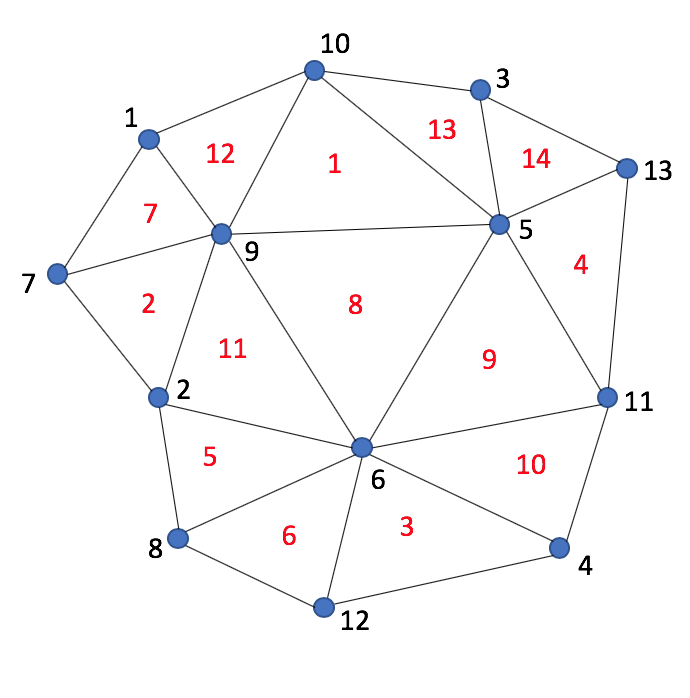
\includegraphics[width=\linewidth]{Fig_split_triangle_01.png}
    \caption{}
  \end{subfigure}
  \begin{subfigure}[b]{0.4\linewidth}
    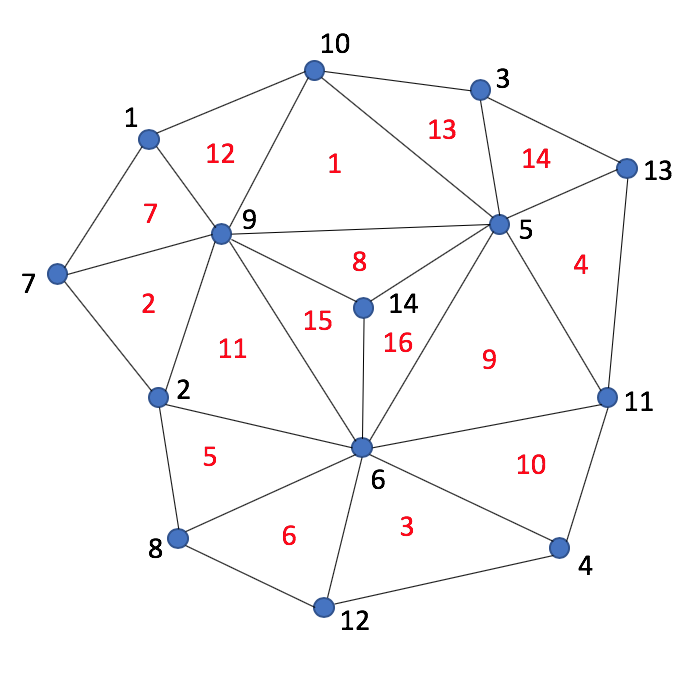
\includegraphics[width=\linewidth]{Fig_split_triangle_02.png}
    \caption{}
  \end{subfigure}
  \begin{subfigure}[b]{0.4\linewidth}
    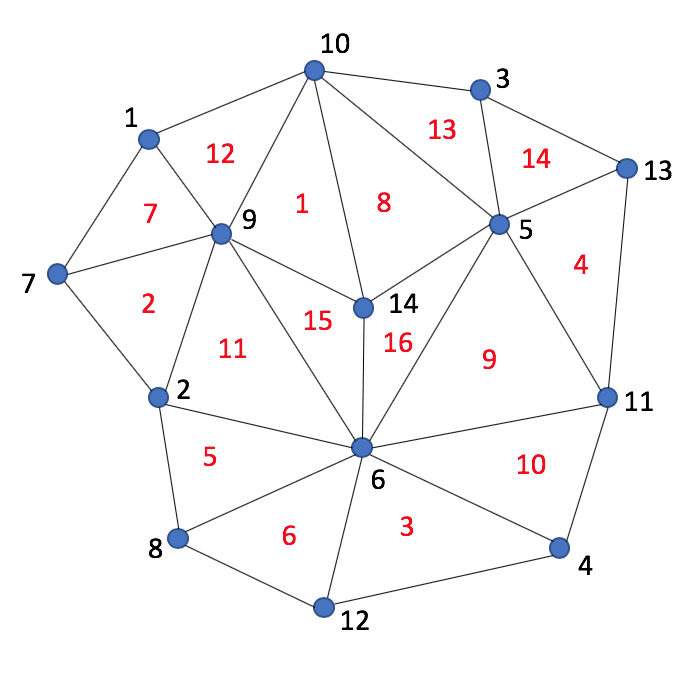
\includegraphics[width=\linewidth]{Fig_split_triangle_03.png}
    \caption{}
  \end{subfigure}
  \begin{subfigure}[b]{0.4\linewidth}
    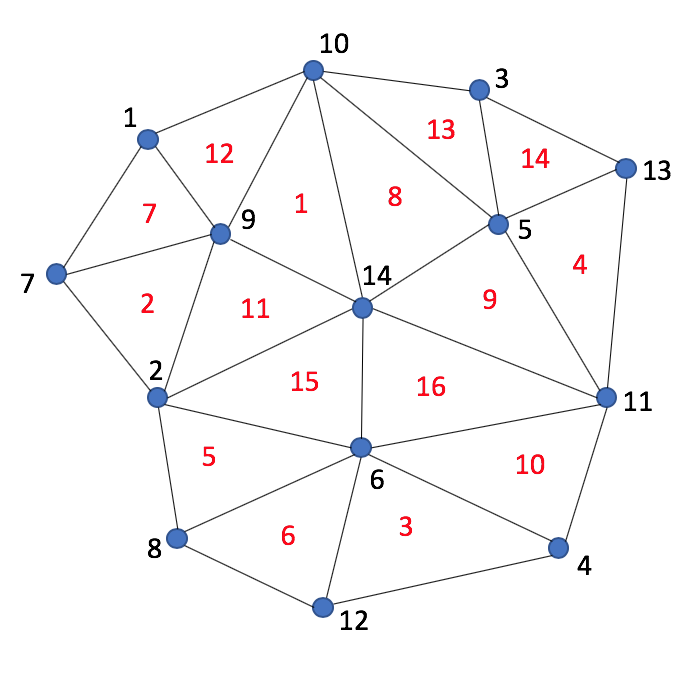
\includegraphics[width=\linewidth]{Fig_split_triangle_04.png}
    \caption{}
  \end{subfigure}
  \caption{(a) Triangle 8 is marked for splitting. (b) A new vertex is added at the circumcentre of triangle 8, replacing it by three new triangles. (c) New triangle pair 8-1 is found to violate the local Delaunay criterion, and is flipped. (d) New triangle pairs 15-11 and 16-9 were also flipped; the mesh now once again is a Delaunay triangulation.}
\end{figure}

In UFEMISM, Ruppert's algorithm has been extended to include more conditions that can cause a triangle to be marked as "bad" than just the smallest internal angle, which are based on the ice model data. Currently, the following conditions are included:

\begin{table}[H]
  \begin{center}
    \caption{mesh refinement conditions}
    \begin{tabular}{ m{10em}| m{40em} } 
      \textbf{config parameter} & \textbf{Description: triangle is marked as bad if...}\\
      \hline
      \textsc{alpha\textunderscore min} & ...any of its three internal angles is smaller than this value (original condition in Ruppert's algorithm).\\
      \textsc{res\textunderscore max} & ...any of its three sides exceeds 2 * this length.\\
      \textsc{res\textunderscore max\textunderscore gl} & ...any of its three sides exceeds 2 * this length and the grounding line passes through it.\\
      \textsc{res\textunderscore max\textunderscore cf} & ...any of its three sides exceeds 2 * this length and the calving front passes through it.\\
      \textsc{res\textunderscore max\textunderscore margin} & ...any of its three sides exceeds 2 * this length and the ice margin passes through it.\\
      \textsc{res\textunderscore max\textunderscore coast} & ...any of its three sides exceeds 2 * this length and the coastline passes through it.\\
      \textsc{poi\textunderscore resolutions} & ...any of its three sides exceeds 2 * this length and it contains a POI.\\
    \end{tabular}
  \end{center}
\end{table}

The mesh is refined step-wise, with the maximum resolutions being halved in each step. This means that generally, resolution ''contrasts'' (differences in resolution between adjacent vertices) that occur during mesh refinement are less dramatic, and that therefore the maximum number of neighbours of any vertex in the mesh (which, for the final mesh, is limited by the maximum internal angle from Ruppert's algorithm, but can be larger during the refinement process) doesn't become as high as would otherwise be the case. This saves on how much memory needs to be allocated, and also makes mesh alignment (see Sect. XX on mesh generation parallelisation) a lot easier.

\begin{figure}[H] \label{fig:stepwise_refinement}
  \centering
  \begin{subfigure}[b]{0.3\linewidth}
    \includegraphics[width=\linewidth]{Fig_mesh_step_01.png}
    \caption{}
  \end{subfigure}
  \begin{subfigure}[b]{0.3\linewidth}
    \includegraphics[width=\linewidth]{Fig_mesh_step_02.png}
    \caption{}
  \end{subfigure}
  \begin{subfigure}[b]{0.3\linewidth}
    \includegraphics[width=\linewidth]{Fig_mesh_step_03.png}
    \caption{}
  \end{subfigure}
  \begin{subfigure}[b]{0.3\linewidth}
    \includegraphics[width=\linewidth]{Fig_mesh_step_04.png}
    \caption{}
  \end{subfigure}
  \begin{subfigure}[b]{0.3\linewidth}
    \includegraphics[width=\linewidth]{Fig_mesh_step_05.png}
    \caption{}
  \end{subfigure}
  \caption{Step-wise refinement of a mesh, with the maximum resolution decreasing from 200 km (a) to 12.5 km (e).}
\end{figure}

The code that performs this step-wise mesh refinement looks more or less like this:

\begin{lstlisting}

! Initialise the five-vertex dummy mesh
CALL initialise_dummy_mesh( mesh)

res_min_inc = C%res_max * 2._dp

DO WHILE (res_min_inc > C%res_min)

  ! Increase resolution
  res_min_inc = res_min_inc / 2._dp

  ! Determine resolutions of regions of interest
  mesh%res_min = MAX( C%res_min, res_min_inc)
  mesh%res_max_margin = MAX( C%res_max_margin, res_min_inc)
  mesh%res_max_gl = MAX( C%res_max_gl, res_min_inc)
  etc.

  ! Refine the process submesh
  CALL refine_mesh( mesh)

  ! Align with neighbouring submeshes
  CALL align_all_submeshes( mesh)

  ! Split any new triangles (added during alignment) that are too sharp
  CALL refine_submesh_geo_only( mesh)
      
  ! Smooth the submesh using Lloyd' algorithm
  CALL Lloyds_algorithm_single_iteration_submesh( mesh)

END DO

\end{lstlisting}

The meaning of the ''alignment'' step is explained in Sect. XX on the parallelisation of mesh generation. Lloyd's algorithm moves all vertices in a mesh to the geometric centres of their Voronoi cells. Theoretically this is an iterative approach, because moving a vertex alters the shape not only of its own Voronoi cell, but also those of all its neighbours. This procedure tends to ''smooth'' the mesh, resulting in nicer triangles (i.e. with internal angles that get closer to 60 degrees) and lower resolution gradients. This greatly improves the stability of the SOR solver used in the SSA.

\begin{figure}[H] \label{fig:mesh_Lloyds_algorithm}
  \centering
  \begin{subfigure}[b]{0.3\linewidth}
    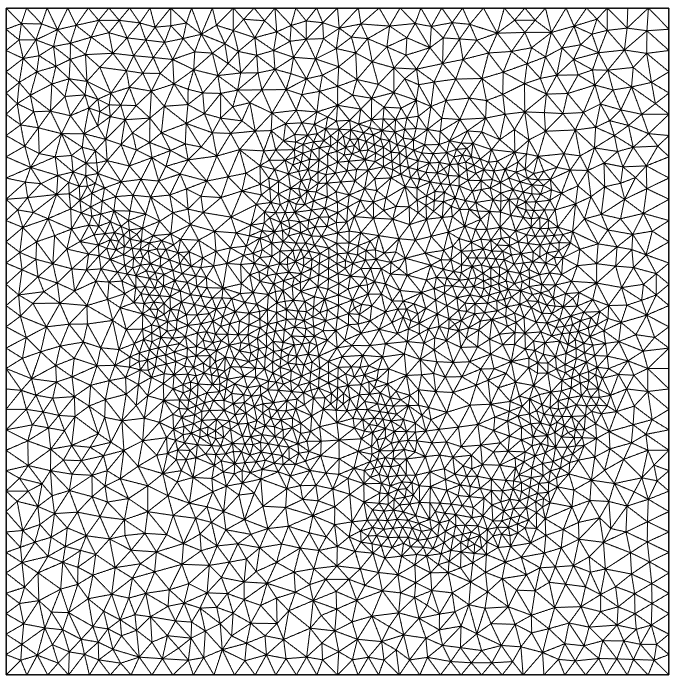
\includegraphics[width=\linewidth]{Fig_mesh_Lloyd_01.png}
    \caption{}
  \end{subfigure}
  \begin{subfigure}[b]{0.3\linewidth}
    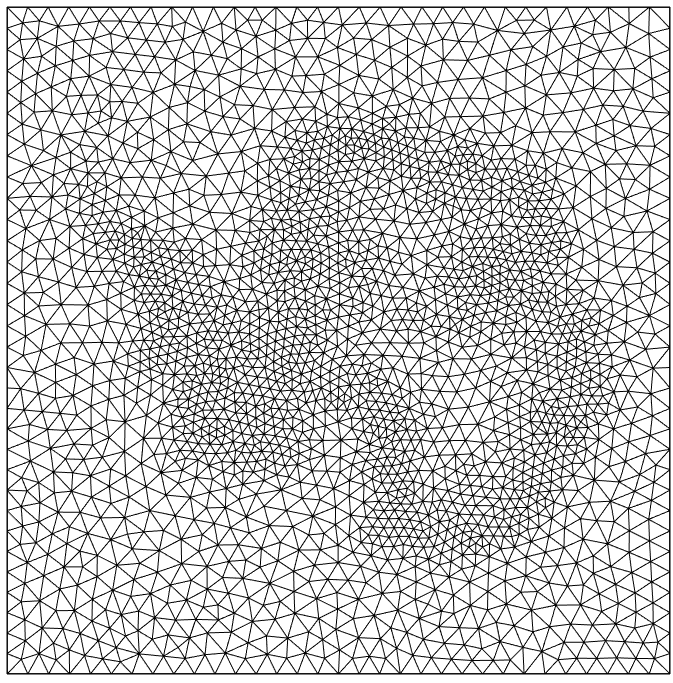
\includegraphics[width=\linewidth]{Fig_mesh_Lloyd_02.png}
    \caption{}
  \end{subfigure}
  \caption{(a) An unsmoothed, 100 km resolution mesh. (b) The same mesh after applying one single iteration of Lloyd's algorithm.}
\end{figure}

If run for infinitely many iterations, the mesh would approach a regular hexagonal structure, since this is the only way for vertices to coincide with the geometric centres of their Voronoi cells. However, to achieve this requires many iterations; only applying a single iteration during each refinement step, as is done here, achieves a good balance between smoothing the mesh without smoothing the resolution gradients too much (which would unnecessarily increase the number of vertices).

\newpage
\subsection{Parallelised mesh generation}

Mesh generation has been parallelised using a form of domain decomposition. Each processor is assigned a portion of the total model domain, and will generate a ''submesh'' for that portion only. Once this is done, the different meshes are ''merged'' to create one single mesh covering the whole model domain.

\begin{figure}[H] \label{fig:submeshes}
  \centering
  \begin{subfigure}[b]{0.15\linewidth}
    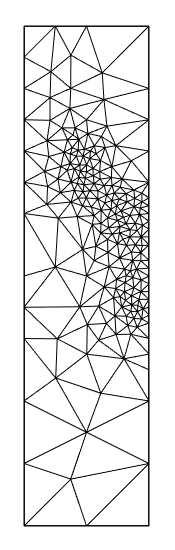
\includegraphics[width=\linewidth]{Fig_submesh1.png}
    \caption{}
  \end{subfigure}
  \begin{subfigure}[b]{0.15\linewidth}
    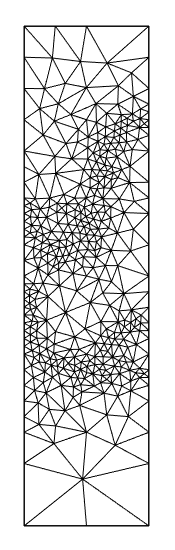
\includegraphics[width=\linewidth]{Fig_submesh2.png}
    \caption{}
  \end{subfigure}
  \begin{subfigure}[b]{0.15\linewidth}
    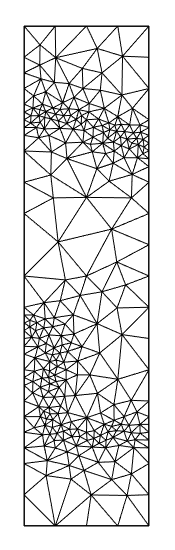
\includegraphics[width=\linewidth]{Fig_submesh3.png}
    \caption{}
  \end{subfigure}
  \begin{subfigure}[b]{0.15\linewidth}
    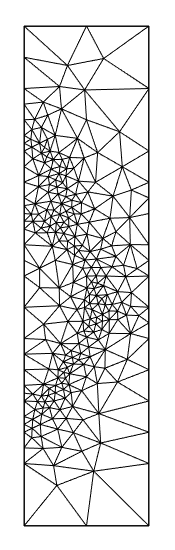
\includegraphics[width=\linewidth]{Fig_submesh4.png}
    \caption{}
  \end{subfigure}
  \caption{Four submeshes for Antarctica.}
\end{figure}

The process of mesh merging hinges on the fact that, when Rupperts algorithm refines a boundary triangle whose circumcentre lies outside the (sub)mesh domain, a new vertex is added at the midpoint of the triangle's segment. This means that boundary vertices always lie at integer sums of power-of-two fractions of a boundary edge (e.g. $\frac{1}{2}$, $\frac{3}{4}$, $\frac{1}{2}+\frac{1}{8}+\frac{13}{64}$, etc.). Looking carefully at submeshes a) and b) in the figure, we can see that many vertices on the eastern boundary of submesh a) lie at the same y-coordinate as vertices on the western boundary of submesh b). These vertices can then be merged. Generally, a small number of vertices on either boundary will have no corresponding vertex on the opposite boundary. During submesh merging, additional vertices are added first to ensure that all vertices on either boundary have corresponding vertices on the opposite boundary (a process called ''submesh alignment'').

\begin{figure}[H] \label{fig:submeshes_align}
  \centering
  \begin{subfigure}[b]{0.3\linewidth}
    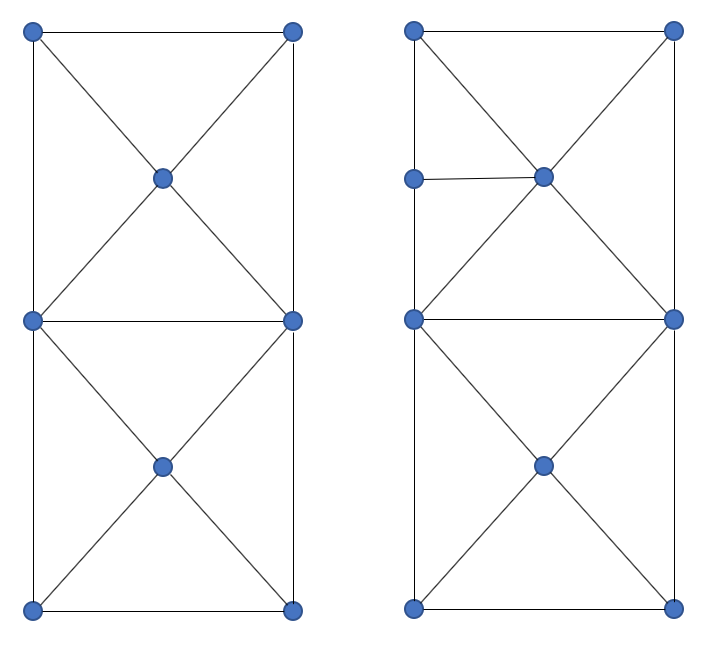
\includegraphics[width=\linewidth]{Fig_mesh_align_01.png}
    \caption{}
  \end{subfigure}
  \begin{subfigure}[b]{0.3\linewidth}
    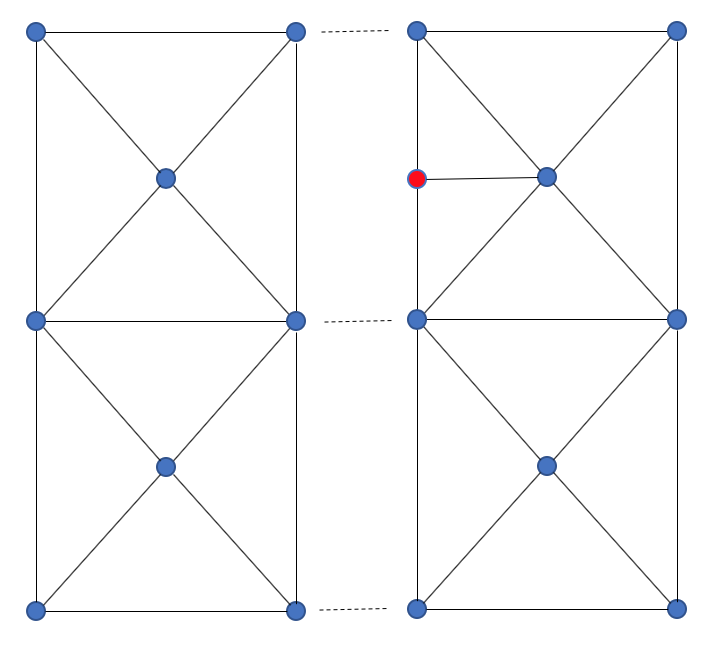
\includegraphics[width=\linewidth]{Fig_mesh_align_02.png}
    \caption{}
  \end{subfigure}
  \begin{subfigure}[b]{0.3\linewidth}
    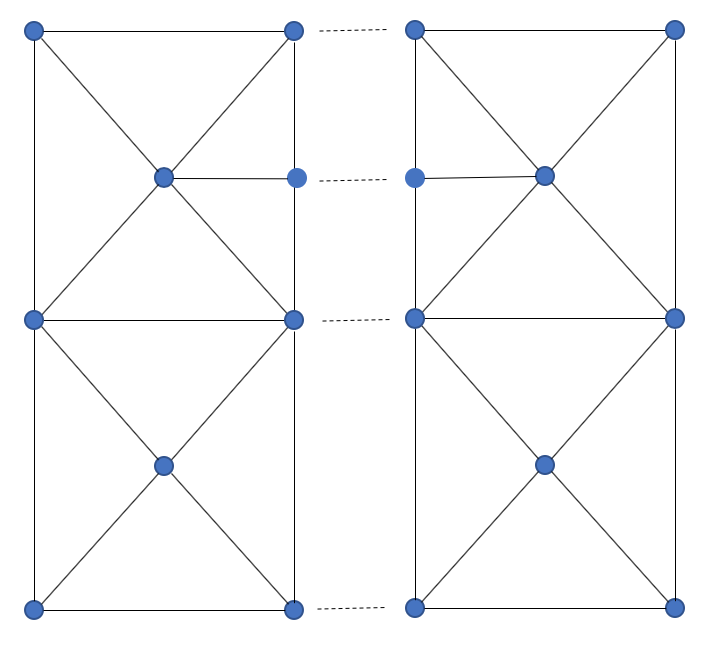
\includegraphics[width=\linewidth]{Fig_mesh_align_03.png}
    \caption{}
  \end{subfigure}
  \caption{Aligning two simple submeshes: a) before, b) a single non-overlapping (red) vertex is detected, c) after.}
\end{figure}

The figure illustrates how two very simple submeshes are aligned. First, the vertices lying on the ''seam'' are checked, and those that overlap are marked. The right-hand submesh has one vertex that doesn't overlap with any vertex in the left-hand submesh. This is remedied by adding a new vertex to the left-hand mesh. All seam vertices now match, and the submeshes can be merged. This is done by merging the overlapping vertices one by one, moving along the seam like a zipper, as illustrated in Fig. Xx.

\begin{figure}[H] \label{fig:submeshes_merge}
  \centering
  \begin{subfigure}[b]{0.2\linewidth}
    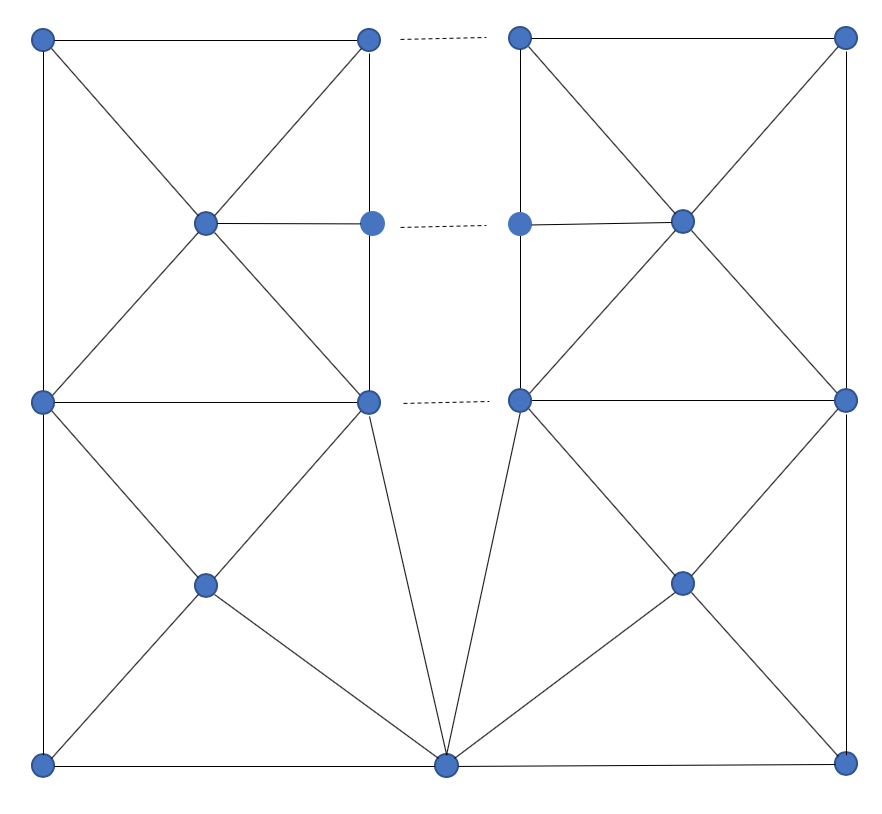
\includegraphics[width=\linewidth]{Fig_mesh_merge_01.png}
    \caption{}
  \end{subfigure}
  \begin{subfigure}[b]{0.2\linewidth}
    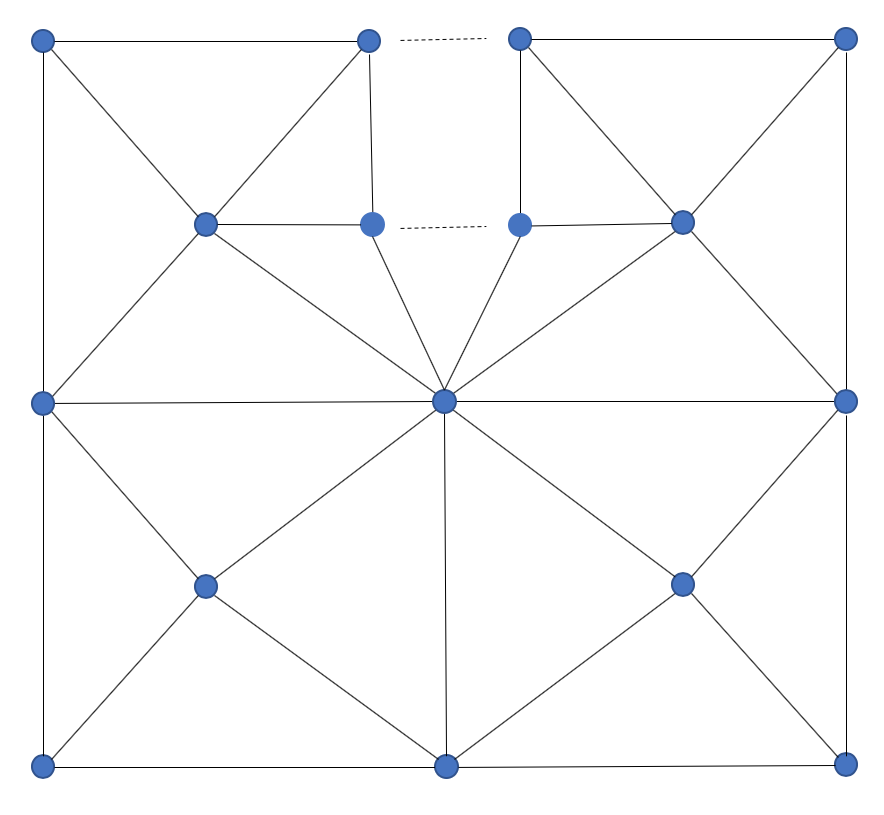
\includegraphics[width=\linewidth]{Fig_mesh_merge_02.png}
    \caption{}
  \end{subfigure}
  \begin{subfigure}[b]{0.2\linewidth}
    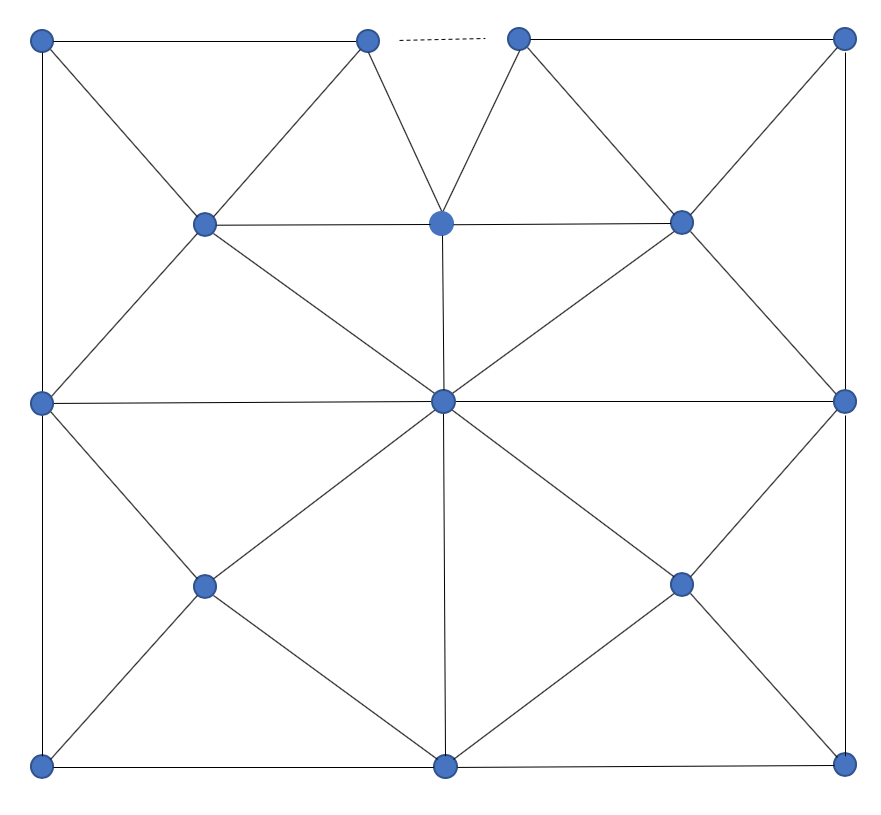
\includegraphics[width=\linewidth]{Fig_mesh_merge_03.png}
    \caption{}
  \end{subfigure}
  \begin{subfigure}[b]{0.2\linewidth}
    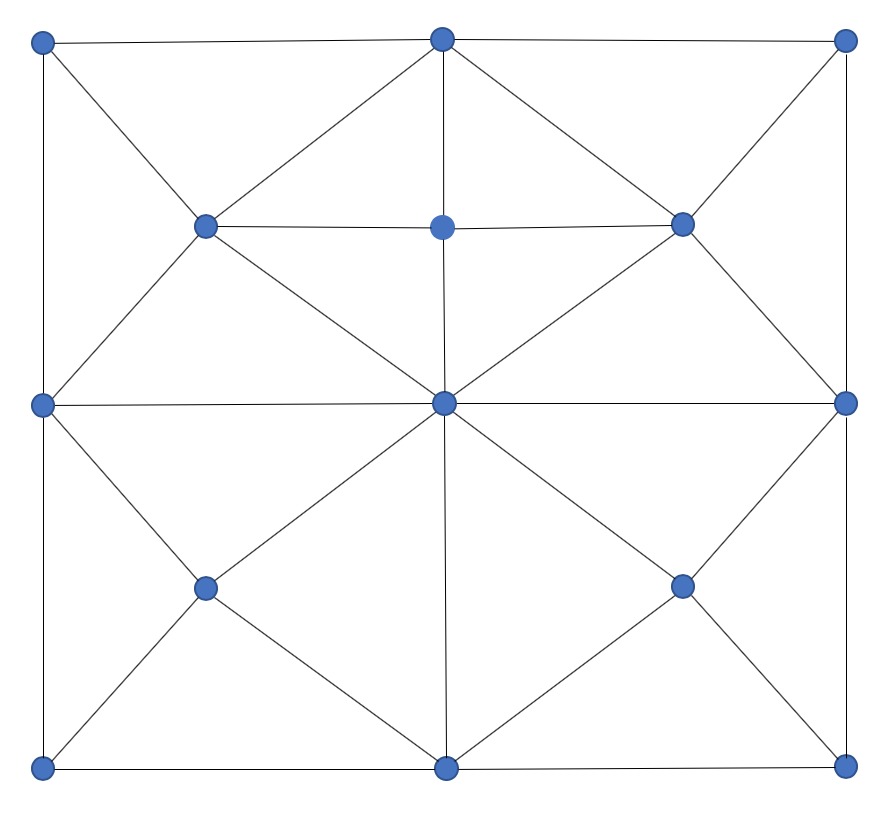
\includegraphics[width=\linewidth]{Fig_mesh_merge_04.png}
    \caption{}
  \end{subfigure}
  \caption{Merging two simple submeshes. Note that no actual deformation is occurring; the vertices along the seam have the same x-ccordinate, and have only been moved apart for this illustration.}
\end{figure}

Since only two submeshes can be merged at a time, submesh merging is an iterative process. For example, the four submeshes in Fig. XX would be merged in two phases. In the first phase, processor a) would be given access to the data of the submesh created by processor b). It allocates new memory that can accomodate the new (merged) submesh ab), and then merges submeshes a) and b) into this new memory. The old memory for submeshes a) and b) is then deallocated. At the same time, processor c) will do the same with submeshes c) and d), creating a new submesh cd). In the second phase, processor a) will merge submeshes ab) and cd) into the final mesh.\\
\\
The four submeshes shown above all have equal domain widths. This is generally not the case; domain widths for mesh generation are determined such that each processor will have (roughly) the same number of vertices. This is done by looking at the vertex coordinates of the previous mesh, which is assumed to be a reasonable approximation of the new mesh.

\newpage
\subsection{Remapping}

Whenever UFEMISM updates the mesh, (some of) the model data must be remapped from the old to the new mesh. Extensive preliminary experiments have shown that the his to be done using a conservative remapping scheme. If, for example, simpler schemes like nearest-neighbour, linear, quadratic, or even cubic interpolation are used, significant errors show up in the results of the schematic benchmark experiments. In the Halfar experiment, the ice thickness tends to ”flatten out”. In the EISMINT experiment, the basal temperature at the ice divide shows a significant warm bias. All of these anomalies disappear when a conservative remapping scheme is used. The conservative remapping scheme developed for UFEMISM is based on the work of Jones (1999). The mathematical principles behind this approach are quite straightforward, but creating an implementation that is both robust and fast enough to handle meshes of hundreds of thousands of vertices was surprisingly difficult.

\subsubsection{Theory}

Let there exist two meshes that both cover the same domain: a ”source” mesh (indicated henceforth by the subscript s) and a ”destination” mesh (subscript d). Suppose the source mesh is the one that existed before a mesh update, and the destination mesh is the newly generated mesh. Let $f(x,y)$ be a continuous function, which is obtained from the discrete data field $f_s$ on the source mesh by using the linear basis functions on the triangles $s^b$, so that $f(x,y)$ is continuous but non-differentiable on the vertices and lines of the source mesh:

\begin{equation} \label{eq:remap_01}
f(x,y) = f_{s^b} + (x - x_{s^b}) {\left( \frac{\partial f}{\partial x} \right)}_{s^b} + (y - y_{s^b}) {\left( \frac{\partial f}{\partial y} \right)}_{s^b}
\end{equation}

Of course, $f_{s^b}$, which is defined on the source triangles, can be obtained from $f_{s^a}$, which is defined on the source vertices, by using the vertex-to-triangle mapping operator $M_{ab}$.\\
\\
The discrete data field $f_{d^a}$ on the destination mesh vertices is found by simply averaging $f(x,y)$ over the Voronoi cells $A_{d^a}$:

\begin{equation} \label{eq:remap_02}
f_{d^a} = \frac{1}{A_{d^a}} \iint_{A_{d^a}} f(x,y) dA
\end{equation}

Substituting \eqref{eq:remap_01} into \eqref{eq:remap_02} yields:

\begin{align} \label{eq:remap_03}
f_{d^a} &= \frac{1}{A_{d^a}} \sum_{s^b} \left[ \iint_{A_{s^v d^a}} \left( f_{s^b} + (x - x_{s^b}) {\left( \frac{\partial f}{\partial x} \right)}_{s^b} + (y - y_{s^b}) {\left( \frac{\partial f}{\partial y} \right)}_{s^b} \right) dA \right], \\
  &= \frac{1}{A_{d^a}} \sum_{s^b} \left[ f_{s^b}  \iint_{A_{s^v d^a}} dA + 
  {\left( \frac{\partial f}{\partial x} \right)}_{s^b} \iint_{A_{s^v d^a}} (x - x_{s^b}) dA + 
  {\left( \frac{\partial f}{\partial y} \right)}_{s^b} \iint_{A_{s^v d^a}} (y - y_{s^b}) dA  \right], \\ 
  &= \frac{1}{A_{d^a}} \sum_{s^b} \left[ \left( f_{s^b}
  - x_{s^b} {\left( \frac{\partial f}{\partial x} \right)}_{s^b}
  - y_{s^b}  {\left( \frac{\partial f}{\partial y} \right)}_{s^b} \right) \iint_{A_{s^v d^a}} dA +
  {\left( \frac{\partial f}{\partial x} \right)}_{s^b} \iint_{A_{s^v d^a}} x dA + 
  {\left( \frac{\partial f}{\partial y} \right)}_{s^b} \iint_{A_{s^v d^a}} y dA 
  \right]
\end{align}

Here, $A_{s^b d^a}$ indicates the area of overlap between the source mesh triangles $s^b$, and the destination mesh Voronoi cells $d^a$.\\
\\
Since the area of overlap $A_{s^b d^a}$ between a Voronoi cell and a triangle will generally be an irregularly-shaped polygon, \eqref{eq:remap_03} is generally not easy to evaluate. However, this problem can be simplified by applying the divergence theorem, rewriting the three surface integrals involved as line integrals:

\begin{align} \label{eq:remap_04}
\iint_A dA &= \oint_C x dy, \\
\iint_A x dA &= - \oint_C xy dx, \\
\iint_A y dA &= \oint_C xy dy.
\end{align}

Substituting these expressions into \eqref{eq:remap_03} yields:

\begin{align} \label{eq:remap_05}
f_{d^a} &= \frac{1}{A_{d^a}} \sum_{s^b} \left[ \left( f_{s^b}
  - x_{s^b} {\left( \frac{\partial f}{\partial x} \right)}_{s^b}
  - y_{s^b}  {\left( \frac{\partial f}{\partial y} \right)}_{s^b} \right) \oint_{C_{s^v d^a}} x dy -
  {\left( \frac{\partial f}{\partial x} \right)}_{s^b} \oint_{C_{s^v d^a}} xy dx + 
  {\left( \frac{\partial f}{\partial y} \right)}_{s^b} \oint_{C_{s^v d^a}} xy dy 
  \right]
\end{align}

This means that, in order to find the remapped value of $f$ on a destination vertex, we need to find all the source triangles overlapping with that vertex' Voronoi cell, and calculate the three line integrals around the perimeter of the area of overlap between the triangle and the Voronoi cell.\\
\\
As can be seen from \eqref{eq:remap_05}, the remapped function $f_{d^a}$ is a linear combination of the source function values $f_{s^b}$ and its derivatives ${\left( \frac{\partial f}{\partial x} \right)}_{s^b}$, ${\left( \frac{\partial f}{\partial y} \right)}_{s^b}$. We can therefore rewrite this expression as a matrix product. First, we define the three matrices $B_{xdy}$, $B_{-xydx}$, and $B_{xydy}$, which describe the line integrals around the areas of overlap between the source triangles $s^b$ and the destination vertices $d^a$:

\begin{align} \label{eq:remap_06}
B_{xdy}^{ij} &= \oint_{C_{d^{ai} s^{bj}}} x dy, \\
B_{-xydx}^{ij} &= - \oint_{C_{d^{ai} s^{bj}}} xy dx, \\
B_{xydy}^{ij} &= \oint_{C_{d^{ai} s^{bj}}} xy dy.
\end{align}

Note that $B_{xdy}^{ij}$ is non-zero if and only if source triangle $j$ and destination Voronoi cell $i$ overlap.\\
\\
These three matrices are combined to yield the three remapping weight matrices $W_0$, $W_{1,x}$, and $W_{1,y}$:

\begin{align} \label{eq:remap_07}
W_0^{ij} &= \frac{B_{xdy}^{ij}}{A_{d^{ai}}}, \\
W_{1,x}^{ij} &= \frac{B_{-xydx}^{ij}}{A_{d^{ai}}} - W_0^{ij} x_{s^{bj}}, \\
W_{1,y}^{ij} &= \frac{B_{xydy}^{ij}}{A_{d^{ai}}} - W_0^{ij} y_{s^{bj}}.
\end{align}

Together, these three matrices represent the linear operation from \eqref{eq:remap_05}:

\begin{equation} \label{eq:remap_08}
f_{d^a} = W_0 f_{s^b} + W_{1,x} {\left( \frac{\partial f}{\partial x} \right)}_{s^b} 
+ W_{1,y} {\left( \frac{\partial f}{\partial y} \right)}_{s^b}
\end{equation}

Typically, the source data field will be defined on the source mesh vertices rather than the triangles. Recalling that both $f_{s^b}$ and its derivatives ${\left( \frac{\partial f}{\partial x} \right)}_{s^b}$, ${\left( \frac{\partial f}{\partial y} \right)}_{s^b}$ can be expressed as linear combinations of $f_{s^a}$ using the operator matrices $M_{ab}$, $M_{\frac{\partial}{\partial x},ab}$, and $M_{\frac{\partial}{\partial y},ab}$, we can define the remapping matrix $M$:

\begin{equation} \label{eq:remap_09}
M = W_0 M_{ab} + W_{1,x} M_{\frac{\partial}{\partial x},ab} + W_{1,y} M_{\frac{\partial}{\partial y},ab}
\end{equation}

The complete remapping operation thus reduces to:

\begin{equation} \label{eq:remap_10}
f_{d^a} = M f_{s^a}
\end{equation}

\subsubsection{Implementation}

In order to calculate the remapping matrix $M$, line integrals need to be calculated around the areas of overlap between all source mesh triangles and destination mesh Voronoi cells. While the line integrals themselves are simple enough when calculated over a straight line segment, determining which triangles overlap with which Voronoi cells is not straightforward. Given the large numbers of vertices and triangles involved in high-resolution meshes (easily several tens of thousands of both), it is necessary to pay attention to computational efficiency, or risk severely slowing down the model.\\
\\
By necessity, the perimeter $C_{d^{ai} s^{bj}}$ of the area of overlap $A_{d^{ai} s^{bj}}$ between source triangle $s^{bj}$ and destination Voronoi cell $d^{ai}$ consists of part of the perimeter $C_{s^{bj}}$ of source triangle $s^{bj}$, and part of the perimeter $C_{d^{ai}}$ of destination Voronoi cell $d^{ai}$. This means that, in order to fill the three $B$-matrices from \eqref{eq:remap_06}, it suffices to integrate once around all source triangles, and once around all destination Voronoi cells.\\
\\
In UFEMISM, this is done using the \textsc{trace\textunderscore line} subroutine. Given a line $pq$, the routine "traces" that line through a mesh, and returns a list of all the Voronoi cells or triangles through which that line passes, and the line integrals for all the individual line segments lying within them. Great care is taken to detect cases where perimeters of source triangles and destination Voronoi cells overlap, to prevent double-counting. By actively "tracing" the line, finding the index of the next triangle or Voronoi cell it crosses into from the connectivity of the one it leaves, instead of performing a mesh-wide search operation every time, computational expense is greatly reduced. Thus, calculating the remapping matrix $M$ only takes a fraction of the computation time required to create a new mesh.

\newpage
\part{References}

\section{Publications using IMAU-ICE}

Berends, C. J., Goelzer, H., Reerink, T. J., Stap., L. B., and van de Wal, R. S. W.: Benchmarking the vertically integrated ice-sheet model IMAU-ICE v2.0, Geosci. Mod. Dev., \textit{in review}, 2022.\\
\\
Stap, L. B., Berends, C. J., Scherrenberg, M. D. W., van de Wal., R. S. W., and Gasson, E. G. W.: Net effect of ice-sheet-atmosphere interactions reduces simulated transient Miocene Antarctic ice sheet variability, The Cryosphere, \textit{in review}, 2022.

\section{Publications using UFEMISM}

Berends, C. J., Goelzer, H., and van de Wal, R. S. W.: The Utrecht Finite Volume Ice-Sheet Model: UFEMISM (version 1.0), Geoscientific Model Development 14, 2443-2470, 2021

\section{Publications using earlier versions (ANICE)}

Bintanja, R., van de Wal, R. S. W., and Oerlemans, J.: Global ice volume variations through the last glacial cycle simulated by a 3-D ice-dynamical model, Quaternary International 95-96, 11-23, 2002\\
\\
Bintanja, R., van de Wal, R., and Oerlemans, J.: Modelled atmospheric temperatures and global sea levels over the past million years, Nature 437, 125-128, 2005\\
\\
de Boer, B., van de Wal, R., Lourens, L. J., Bintanja, R., and Reerink, T. J.: A continuous simulation of global ice volume over the past 1 million years with 3-D ice-sheet models, Climate Dynamics 41, 1365-1384, 2013\\
\\
de Boer, B., Stocchi, P., and van de Wal, R.: A fully coupled 3-D ice-sheet-sea-level model: algorithm and applications, Geoscientific Model Development 7, 2141-2156, 2014a\\
\\
de Boer, B., Lourens, L. J., and van de Wal, R. S. W.: Persistent 400,000-year variability of Antarctic ice volume and the carbon cycle is revealed throughout the Plio-Pleistocene, Nature Communications 5, 2014b\\
\\
de Boer, B., Dolan, A. M., Bernales, J., Gasson, E., Goelzer, H., Golledge, N. R., Sutter, J., Huybrechts, P., Lohmann, G., Rogozhina, I., Abe-Ouchi, A., Saito, F., and van de Wal, R. S. W.: Simulating the Antarctic ice sheet in the Late-Pliocene warm period: PLISMIP-ANT, an ice-sheet model intercomparison project, The Cryosphere 9, 881-903, 2015\\
\\
de Boer, B., Haywood, A. M., Dolan, A. M., Hunter, S. J., and Prescott, C. L.: The Transient Response of Ice Volume to Orbital Forcing During the Warm Late Pliocene, Geophysical Research Letters 44, 10,486-10,494, 2017\\
\\
Berends, C. J. and van de Wal, R. S. W.: A computationally efficient depression-filling algorithm for digital elevation models applied to proglacial lake drainage, Geoscientific Model Development 9, 4451-4460, 2016\\
\\
Berends, C. J., de Boer, B., and van de Wal, R. S. W.: Application of HadCM3@Bristolv1.0 simulations of paleoclimate as forcing for an ice-sheet model, ANICE2.1: set-up and benchmark experiments, Geoscientific Model Development 11, 4657-4675, 2018\\
\\
Berends, C. J., de Boer, B., Dolan, A. M., Hill, D. J., and van de Wal, R. S. W.: Modelling ice sheet evolution and atmospheric CO2 during the Late Pliocene, Climate of the Past 15, 1603-1619, 2019\\
\\
Berends, C. J., de Boer, B., and van de Wal, R. S. W.: Reconstructing the evolution of ice sheets, sea level, and atmospheric CO2 during the past 3.6 million years, Climate of the Past 17, 361-377, 2021

\section{Other}

\end{document}
